\chapter{Complete Tokyo Site Evidence}\label{ch:tokyo-atlas}

\section{Site-level observations and decision states}

Each section contains the four retained photographs for one selected physical site and every A--D decision for its four cross-time protocols. The panels expose reference coverage directly. Front/day, left/day, front/night and front/sunset metadata define the views; their identity labels do not supply an independently measured planar transform or metric camera pose. The source imagery is from Tokyo 24/7 \citep{torii2015}, but these tables belong to the custom query-to-query subset.

R is the rank of the correct identity in the saved complete ranking. Decision states are correct, wrong, rejected and ranking only. A wrong state means geometric acceptance of another place; it does not mean every correspondence is known to be false. Global retrieval has no acceptance or inlier-count claim. Protocol labels D--D, D--N, N--D and D--S mean day to changed-direction day, day to night, night to day and day to sunset.

\section{Site tokyo\_000}

This site contributes four real photographs and four labelled retrieval queries. Each protocol uses one of the photographs as its query and the condition-specific 24-site gallery defined in the frozen benchmark. Reusing a site across protocols produces paired condition observations, not four new geographic locations.

\begin{figure}[H]\centering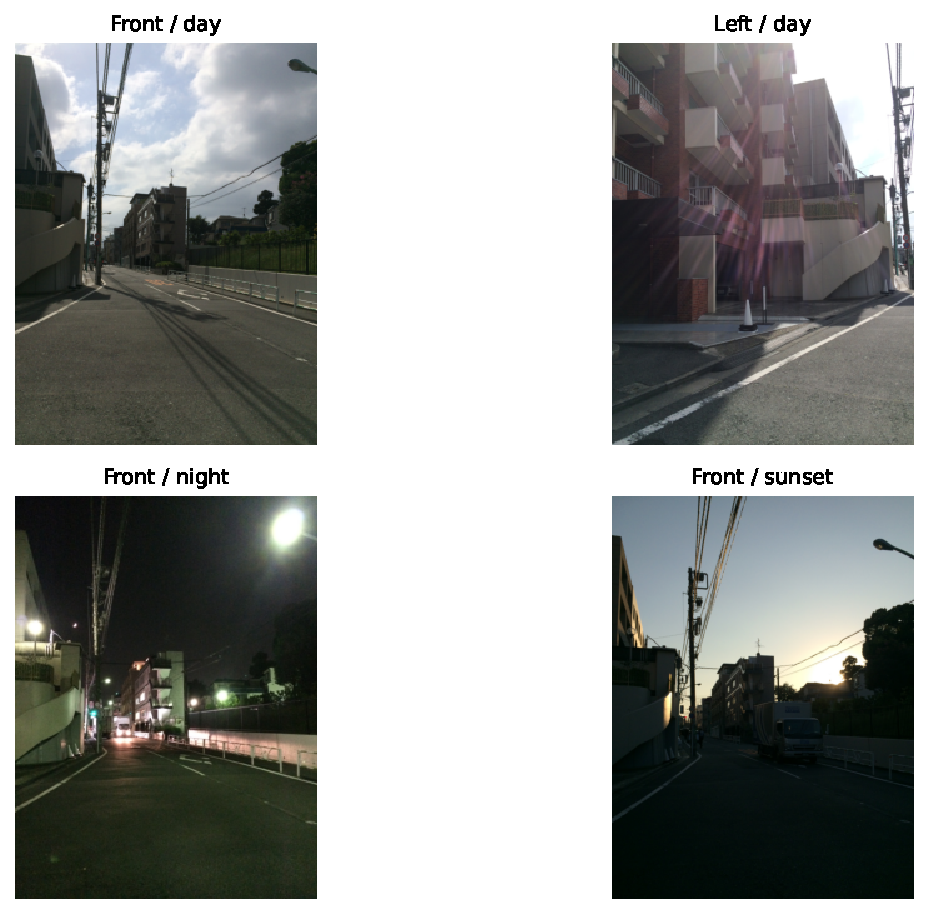
\includegraphics[width=.92\textwidth]{evidence/tokyo_00.pdf}
\caption{All retained photographs for tokyo\_000.}\label{fig:tokyo-scene-0}\end{figure}

\begin{table}[H]\centering\small
\caption{All main-method decisions for tokyo\_000.}\label{tab:tokyo-site-0}
\begin{tabular}{llrlr}\toprule
Protocol & Method & R & Decision & Selected inliers \\
\midrule
D--D & SIFT & 1 & correct & 62 \\
D--D & SP+LG & 1 & correct & 106 \\
D--D & Global & 6 & ranking only & -- \\
D--D & Full & 6 & rejected & 0 \\
D--N & SIFT & 3 & rejected & 0 \\
D--N & SP+LG & 1 & correct & 163 \\
D--N & Global & 1 & ranking only & -- \\
D--N & Full & 1 & correct & 163 \\
N--D & SIFT & 3 & rejected & 0 \\
N--D & SP+LG & 1 & correct & 168 \\
N--D & Global & 1 & ranking only & -- \\
N--D & Full & 1 & correct & 168 \\
D--S & SIFT & 1 & correct & 31 \\
D--S & SP+LG & 1 & correct & 194 \\
D--S & Global & 1 & ranking only & -- \\
D--S & Full & 1 & correct & 194 \\
\bottomrule\end{tabular}\end{table}


Across these four protocols, SIFT correctly verifies 2, exhaustive SP+LG 4, and the full hierarchy 3 of the four queries. The full hierarchy makes 0 wrong-place acceptances and 1 rejection. These counts separate a missing anchor from an incorrectly accepted identity; the latter is the more direct location-association failure.

For this site, the full-pipeline changed-direction daytime query is rejected, while its front-facing day-to-night query is correctly verified. This paired observation should be read with the photographs and the rank column. It does not identify the causal effect of illumination alone, because overlap and view direction also change between the protocols. No corner-error or metric-pose value is inferred from a correct place label.

\section{Site tokyo\_001}

This site contributes four real photographs and four labelled retrieval queries. Each protocol uses one of the photographs as its query and the condition-specific 24-site gallery defined in the frozen benchmark. Reusing a site across protocols produces paired condition observations, not four new geographic locations.

\begin{figure}[H]\centering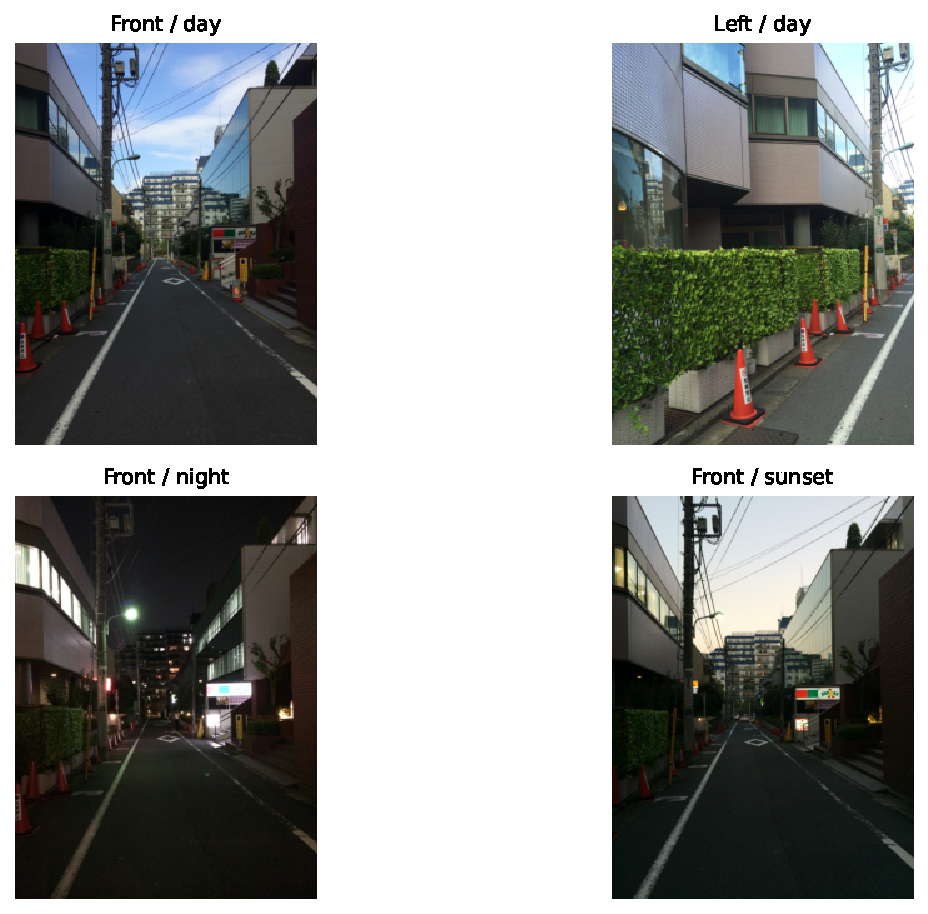
\includegraphics[width=.92\textwidth]{evidence/tokyo_01.pdf}
\caption{All retained photographs for tokyo\_001.}\label{fig:tokyo-scene-1}\end{figure}

\begin{table}[H]\centering\small
\caption{All main-method decisions for tokyo\_001.}\label{tab:tokyo-site-1}
\begin{tabular}{llrlr}\toprule
Protocol & Method & R & Decision & Selected inliers \\
\midrule
D--D & SIFT & 1 & correct & 69 \\
D--D & SP+LG & 1 & correct & 129 \\
D--D & Global & 1 & ranking only & -- \\
D--D & Full & 1 & correct & 129 \\
D--N & SIFT & 1 & correct & 17 \\
D--N & SP+LG & 1 & correct & 199 \\
D--N & Global & 1 & ranking only & -- \\
D--N & Full & 1 & correct & 199 \\
N--D & SIFT & 1 & correct & 17 \\
N--D & SP+LG & 1 & correct & 176 \\
N--D & Global & 1 & ranking only & -- \\
N--D & Full & 1 & correct & 176 \\
D--S & SIFT & 1 & correct & 132 \\
D--S & SP+LG & 1 & correct & 280 \\
D--S & Global & 1 & ranking only & -- \\
D--S & Full & 1 & correct & 280 \\
\bottomrule\end{tabular}\end{table}


Across these four protocols, SIFT correctly verifies 4, exhaustive SP+LG 4, and the full hierarchy 4 of the four queries. The full hierarchy makes 0 wrong-place acceptances and 0 rejections. These counts separate a missing anchor from an incorrectly accepted identity; the latter is the more direct location-association failure.

For this site, the full-pipeline changed-direction daytime query is correctly verified, while its front-facing day-to-night query is correctly verified. This paired observation should be read with the photographs and the rank column. It does not identify the causal effect of illumination alone, because overlap and view direction also change between the protocols. No corner-error or metric-pose value is inferred from a correct place label.

\section{Site tokyo\_002}

This site contributes four real photographs and four labelled retrieval queries. Each protocol uses one of the photographs as its query and the condition-specific 24-site gallery defined in the frozen benchmark. Reusing a site across protocols produces paired condition observations, not four new geographic locations.

\begin{figure}[H]\centering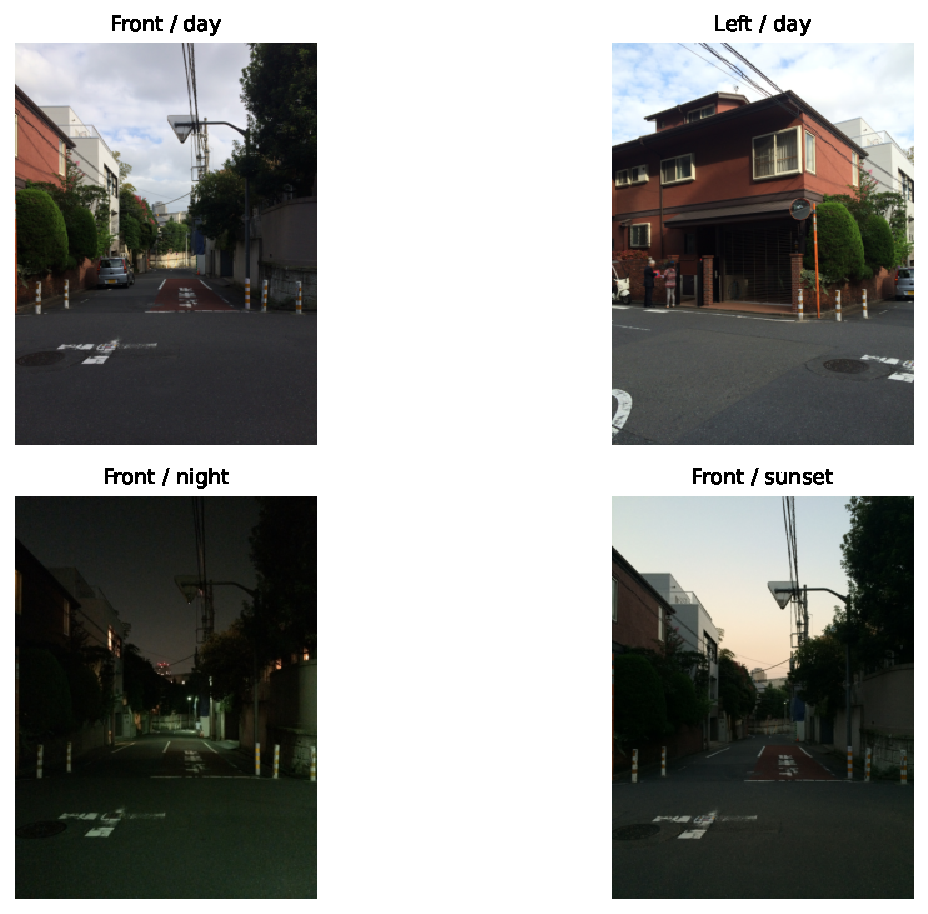
\includegraphics[width=.92\textwidth]{evidence/tokyo_02.pdf}
\caption{All retained photographs for tokyo\_002.}\label{fig:tokyo-scene-2}\end{figure}

\begin{table}[H]\centering\small
\caption{All main-method decisions for tokyo\_002.}\label{tab:tokyo-site-2}
\begin{tabular}{llrlr}\toprule
Protocol & Method & R & Decision & Selected inliers \\
\midrule
D--D & SIFT & 1 & correct & 73 \\
D--D & SP+LG & 1 & correct & 105 \\
D--D & Global & 1 & ranking only & -- \\
D--D & Full & 1 & correct & 105 \\
D--N & SIFT & 1 & correct & 32 \\
D--N & SP+LG & 1 & correct & 176 \\
D--N & Global & 1 & ranking only & -- \\
D--N & Full & 1 & correct & 176 \\
N--D & SIFT & 1 & correct & 30 \\
N--D & SP+LG & 1 & correct & 202 \\
N--D & Global & 1 & ranking only & -- \\
N--D & Full & 1 & correct & 202 \\
D--S & SIFT & 1 & correct & 119 \\
D--S & SP+LG & 1 & correct & 315 \\
D--S & Global & 1 & ranking only & -- \\
D--S & Full & 1 & correct & 315 \\
\bottomrule\end{tabular}\end{table}


Across these four protocols, SIFT correctly verifies 4, exhaustive SP+LG 4, and the full hierarchy 4 of the four queries. The full hierarchy makes 0 wrong-place acceptances and 0 rejections. These counts separate a missing anchor from an incorrectly accepted identity; the latter is the more direct location-association failure.

For this site, the full-pipeline changed-direction daytime query is correctly verified, while its front-facing day-to-night query is correctly verified. This paired observation should be read with the photographs and the rank column. It does not identify the causal effect of illumination alone, because overlap and view direction also change between the protocols. No corner-error or metric-pose value is inferred from a correct place label.

\section{Site tokyo\_003}

This site contributes four real photographs and four labelled retrieval queries. Each protocol uses one of the photographs as its query and the condition-specific 24-site gallery defined in the frozen benchmark. Reusing a site across protocols produces paired condition observations, not four new geographic locations.

\begin{figure}[H]\centering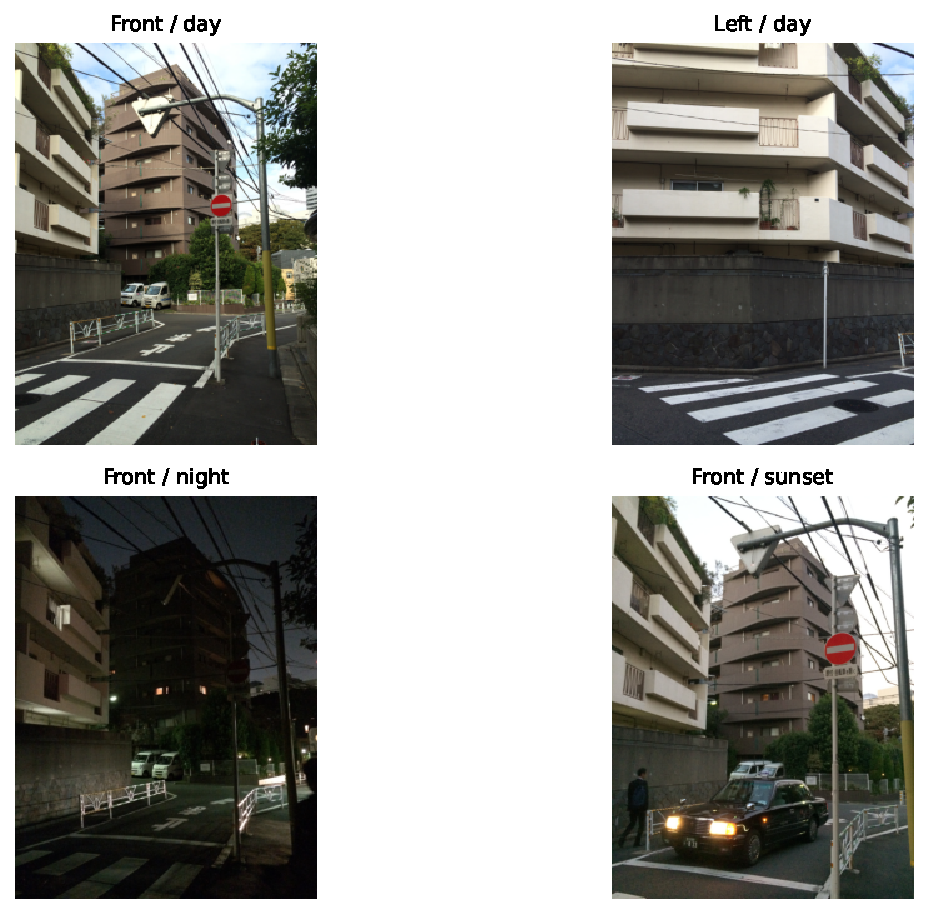
\includegraphics[width=.92\textwidth]{evidence/tokyo_03.pdf}
\caption{All retained photographs for tokyo\_003.}\label{fig:tokyo-scene-3}\end{figure}

\begin{table}[H]\centering\small
\caption{All main-method decisions for tokyo\_003.}\label{tab:tokyo-site-3}
\begin{tabular}{llrlr}\toprule
Protocol & Method & R & Decision & Selected inliers \\
\midrule
D--D & SIFT & 1 & rejected & 0 \\
D--D & SP+LG & 1 & correct & 73 \\
D--D & Global & 1 & ranking only & -- \\
D--D & Full & 1 & correct & 73 \\
D--N & SIFT & 1 & correct & 15 \\
D--N & SP+LG & 1 & correct & 168 \\
D--N & Global & 1 & ranking only & -- \\
D--N & Full & 1 & correct & 168 \\
N--D & SIFT & 1 & correct & 20 \\
N--D & SP+LG & 1 & correct & 167 \\
N--D & Global & 1 & ranking only & -- \\
N--D & Full & 1 & correct & 167 \\
D--S & SIFT & 1 & correct & 13 \\
D--S & SP+LG & 1 & correct & 101 \\
D--S & Global & 1 & ranking only & -- \\
D--S & Full & 1 & correct & 101 \\
\bottomrule\end{tabular}\end{table}


Across these four protocols, SIFT correctly verifies 3, exhaustive SP+LG 4, and the full hierarchy 4 of the four queries. The full hierarchy makes 0 wrong-place acceptances and 0 rejections. These counts separate a missing anchor from an incorrectly accepted identity; the latter is the more direct location-association failure.

For this site, the full-pipeline changed-direction daytime query is correctly verified, while its front-facing day-to-night query is correctly verified. This paired observation should be read with the photographs and the rank column. It does not identify the causal effect of illumination alone, because overlap and view direction also change between the protocols. No corner-error or metric-pose value is inferred from a correct place label.

\section{Site tokyo\_004}

This site contributes four real photographs and four labelled retrieval queries. Each protocol uses one of the photographs as its query and the condition-specific 24-site gallery defined in the frozen benchmark. Reusing a site across protocols produces paired condition observations, not four new geographic locations.

\begin{figure}[H]\centering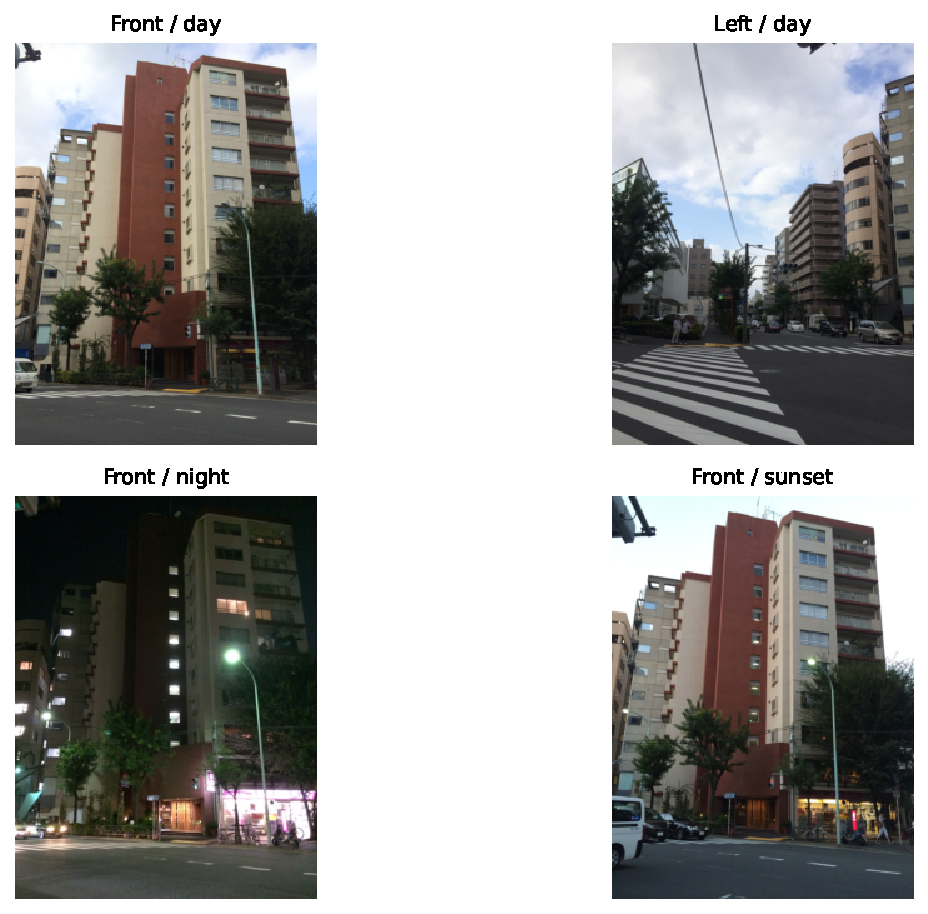
\includegraphics[width=.92\textwidth]{evidence/tokyo_04.pdf}
\caption{All retained photographs for tokyo\_004.}\label{fig:tokyo-scene-4}\end{figure}

\begin{table}[H]\centering\small
\caption{All main-method decisions for tokyo\_004.}\label{tab:tokyo-site-4}
\begin{tabular}{llrlr}\toprule
Protocol & Method & R & Decision & Selected inliers \\
\midrule
D--D & SIFT & 1 & correct & 28 \\
D--D & SP+LG & 1 & correct & 78 \\
D--D & Global & 1 & ranking only & -- \\
D--D & Full & 1 & correct & 78 \\
D--N & SIFT & 2 & rejected & 0 \\
D--N & SP+LG & 1 & correct & 211 \\
D--N & Global & 1 & ranking only & -- \\
D--N & Full & 1 & correct & 211 \\
N--D & SIFT & 7 & rejected & 0 \\
N--D & SP+LG & 1 & correct & 202 \\
N--D & Global & 1 & ranking only & -- \\
N--D & Full & 1 & correct & 202 \\
D--S & SIFT & 1 & correct & 144 \\
D--S & SP+LG & 1 & correct & 328 \\
D--S & Global & 1 & ranking only & -- \\
D--S & Full & 1 & correct & 328 \\
\bottomrule\end{tabular}\end{table}


Across these four protocols, SIFT correctly verifies 2, exhaustive SP+LG 4, and the full hierarchy 4 of the four queries. The full hierarchy makes 0 wrong-place acceptances and 0 rejections. These counts separate a missing anchor from an incorrectly accepted identity; the latter is the more direct location-association failure.

For this site, the full-pipeline changed-direction daytime query is correctly verified, while its front-facing day-to-night query is correctly verified. This paired observation should be read with the photographs and the rank column. It does not identify the causal effect of illumination alone, because overlap and view direction also change between the protocols. No corner-error or metric-pose value is inferred from a correct place label.

\section{Site tokyo\_005}

This site contributes four real photographs and four labelled retrieval queries. Each protocol uses one of the photographs as its query and the condition-specific 24-site gallery defined in the frozen benchmark. Reusing a site across protocols produces paired condition observations, not four new geographic locations.

\begin{figure}[H]\centering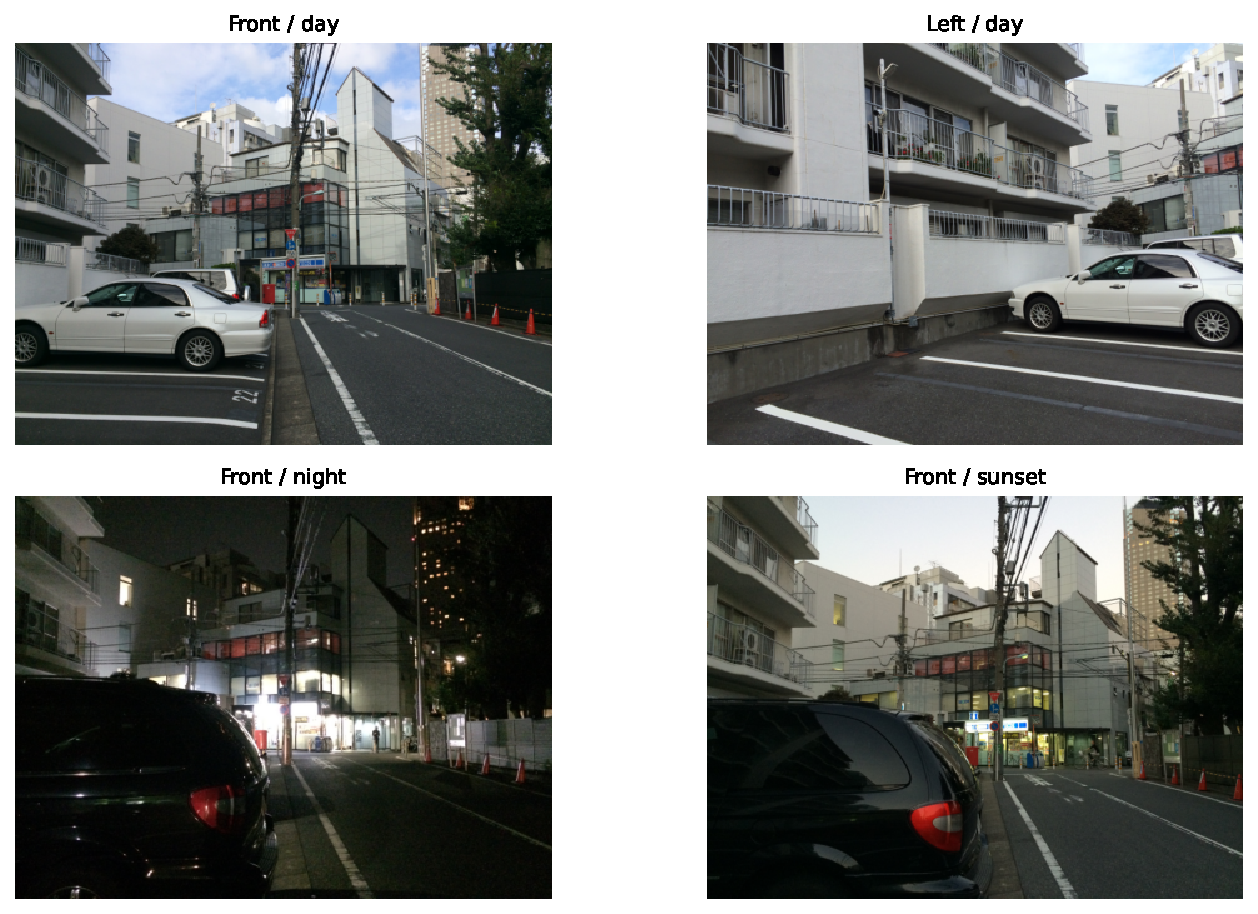
\includegraphics[width=.92\textwidth]{evidence/tokyo_05.pdf}
\caption{All retained photographs for tokyo\_005.}\label{fig:tokyo-scene-5}\end{figure}

\begin{table}[H]\centering\small
\caption{All main-method decisions for tokyo\_005.}\label{tab:tokyo-site-5}
\begin{tabular}{llrlr}\toprule
Protocol & Method & R & Decision & Selected inliers \\
\midrule
D--D & SIFT & 1 & correct & 60 \\
D--D & SP+LG & 1 & correct & 166 \\
D--D & Global & 1 & ranking only & -- \\
D--D & Full & 1 & correct & 166 \\
D--N & SIFT & 11 & rejected & 0 \\
D--N & SP+LG & 1 & correct & 172 \\
D--N & Global & 1 & ranking only & -- \\
D--N & Full & 1 & correct & 172 \\
N--D & SIFT & 8 & rejected & 0 \\
N--D & SP+LG & 1 & correct & 178 \\
N--D & Global & 1 & ranking only & -- \\
N--D & Full & 1 & correct & 178 \\
D--S & SIFT & 1 & correct & 98 \\
D--S & SP+LG & 1 & correct & 282 \\
D--S & Global & 1 & ranking only & -- \\
D--S & Full & 1 & correct & 282 \\
\bottomrule\end{tabular}\end{table}


Across these four protocols, SIFT correctly verifies 2, exhaustive SP+LG 4, and the full hierarchy 4 of the four queries. The full hierarchy makes 0 wrong-place acceptances and 0 rejections. These counts separate a missing anchor from an incorrectly accepted identity; the latter is the more direct location-association failure.

For this site, the full-pipeline changed-direction daytime query is correctly verified, while its front-facing day-to-night query is correctly verified. This paired observation should be read with the photographs and the rank column. It does not identify the causal effect of illumination alone, because overlap and view direction also change between the protocols. No corner-error or metric-pose value is inferred from a correct place label.

\section{Site tokyo\_006}

This site contributes four real photographs and four labelled retrieval queries. Each protocol uses one of the photographs as its query and the condition-specific 24-site gallery defined in the frozen benchmark. Reusing a site across protocols produces paired condition observations, not four new geographic locations.

\begin{figure}[H]\centering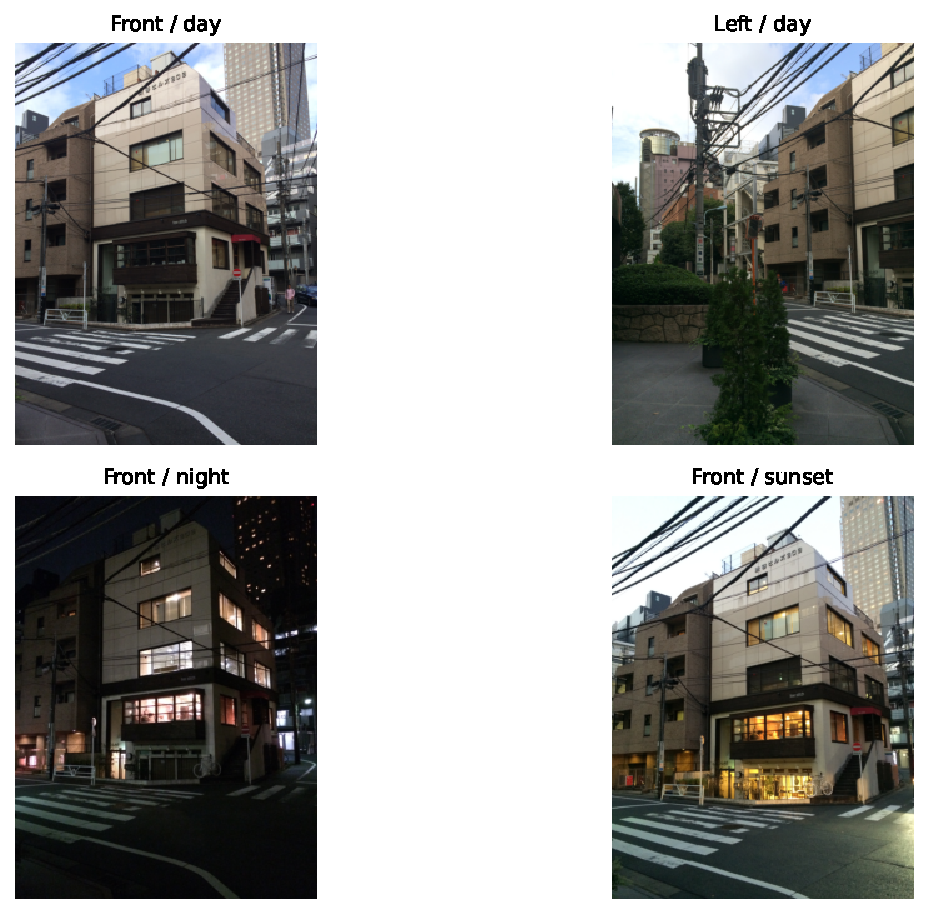
\includegraphics[width=.92\textwidth]{evidence/tokyo_06.pdf}
\caption{All retained photographs for tokyo\_006.}\label{fig:tokyo-scene-6}\end{figure}

\begin{table}[H]\centering\small
\caption{All main-method decisions for tokyo\_006.}\label{tab:tokyo-site-6}
\begin{tabular}{llrlr}\toprule
Protocol & Method & R & Decision & Selected inliers \\
\midrule
D--D & SIFT & 1 & correct & 40 \\
D--D & SP+LG & 1 & correct & 137 \\
D--D & Global & 1 & ranking only & -- \\
D--D & Full & 1 & correct & 137 \\
D--N & SIFT & 3 & rejected & 0 \\
D--N & SP+LG & 1 & correct & 243 \\
D--N & Global & 1 & ranking only & -- \\
D--N & Full & 1 & correct & 243 \\
N--D & SIFT & 1 & rejected & 0 \\
N--D & SP+LG & 1 & correct & 244 \\
N--D & Global & 1 & ranking only & -- \\
N--D & Full & 1 & correct & 244 \\
D--S & SIFT & 1 & correct & 43 \\
D--S & SP+LG & 1 & correct & 275 \\
D--S & Global & 1 & ranking only & -- \\
D--S & Full & 1 & correct & 275 \\
\bottomrule\end{tabular}\end{table}


Across these four protocols, SIFT correctly verifies 2, exhaustive SP+LG 4, and the full hierarchy 4 of the four queries. The full hierarchy makes 0 wrong-place acceptances and 0 rejections. These counts separate a missing anchor from an incorrectly accepted identity; the latter is the more direct location-association failure.

For this site, the full-pipeline changed-direction daytime query is correctly verified, while its front-facing day-to-night query is correctly verified. This paired observation should be read with the photographs and the rank column. It does not identify the causal effect of illumination alone, because overlap and view direction also change between the protocols. No corner-error or metric-pose value is inferred from a correct place label.

\section{Site tokyo\_007}

This site contributes four real photographs and four labelled retrieval queries. Each protocol uses one of the photographs as its query and the condition-specific 24-site gallery defined in the frozen benchmark. Reusing a site across protocols produces paired condition observations, not four new geographic locations.

\begin{figure}[H]\centering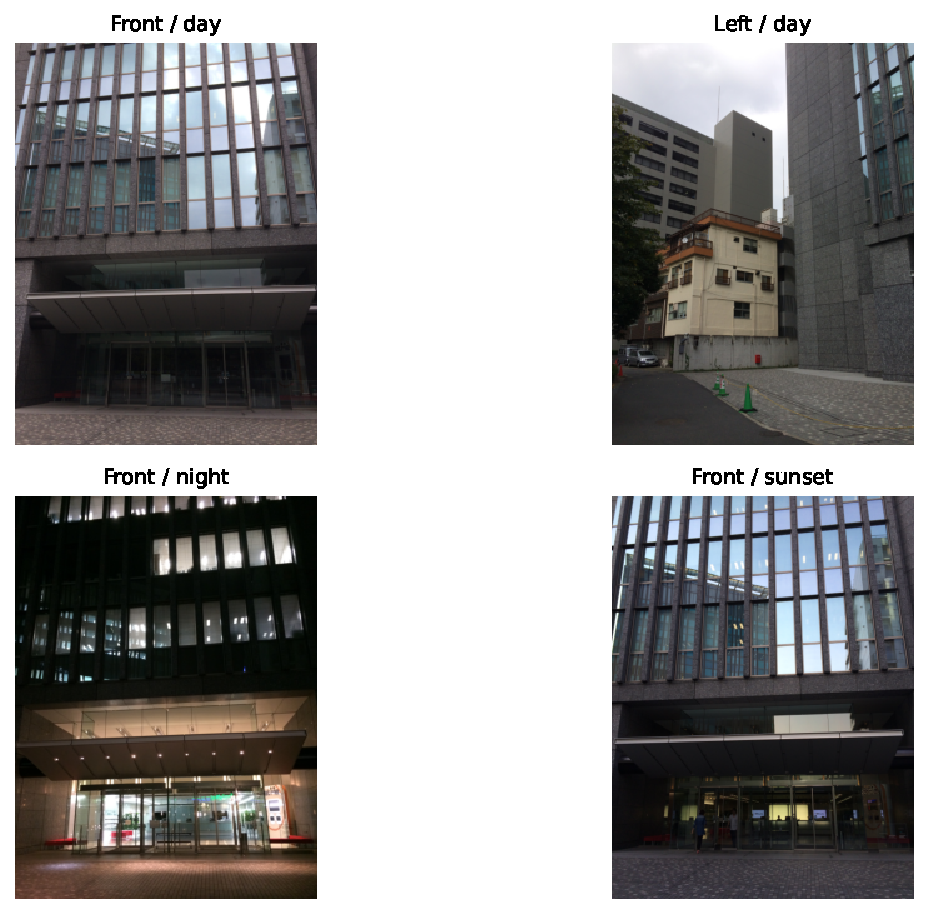
\includegraphics[width=.92\textwidth]{evidence/tokyo_07.pdf}
\caption{All retained photographs for tokyo\_007.}\label{fig:tokyo-scene-7}\end{figure}

\begin{table}[H]\centering\small
\caption{All main-method decisions for tokyo\_007.}\label{tab:tokyo-site-7}
\begin{tabular}{llrlr}\toprule
Protocol & Method & R & Decision & Selected inliers \\
\midrule
D--D & SIFT & 1 & rejected & 0 \\
D--D & SP+LG & 1 & correct & 34 \\
D--D & Global & 16 & ranking only & -- \\
D--D & Full & 16 & wrong & 13 \\
D--N & SIFT & 1 & rejected & 0 \\
D--N & SP+LG & 1 & correct & 87 \\
D--N & Global & 1 & ranking only & -- \\
D--N & Full & 1 & correct & 87 \\
N--D & SIFT & 3 & rejected & 0 \\
N--D & SP+LG & 1 & correct & 88 \\
N--D & Global & 1 & ranking only & -- \\
N--D & Full & 1 & correct & 88 \\
D--S & SIFT & 1 & correct & 37 \\
D--S & SP+LG & 1 & correct & 280 \\
D--S & Global & 1 & ranking only & -- \\
D--S & Full & 1 & correct & 280 \\
\bottomrule\end{tabular}\end{table}


Across these four protocols, SIFT correctly verifies 1, exhaustive SP+LG 4, and the full hierarchy 3 of the four queries. The full hierarchy makes 1 wrong-place acceptance and 0 rejections. These counts separate a missing anchor from an incorrectly accepted identity; the latter is the more direct location-association failure.

For this site, the full-pipeline changed-direction daytime query is accepted at the wrong place, while its front-facing day-to-night query is correctly verified. This paired observation should be read with the photographs and the rank column. It does not identify the causal effect of illumination alone, because overlap and view direction also change between the protocols. No corner-error or metric-pose value is inferred from a correct place label.

\section{Site tokyo\_008}

This site contributes four real photographs and four labelled retrieval queries. Each protocol uses one of the photographs as its query and the condition-specific 24-site gallery defined in the frozen benchmark. Reusing a site across protocols produces paired condition observations, not four new geographic locations.

\begin{figure}[H]\centering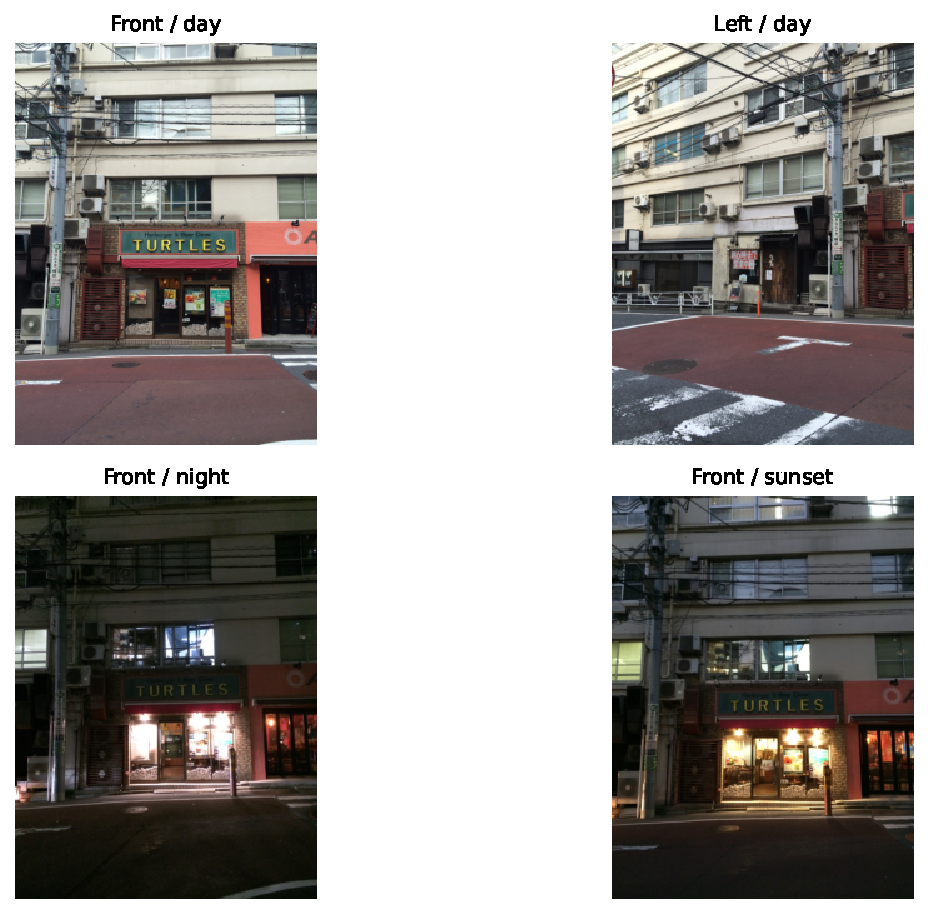
\includegraphics[width=.92\textwidth]{evidence/tokyo_08.pdf}
\caption{All retained photographs for tokyo\_008.}\label{fig:tokyo-scene-8}\end{figure}

\begin{table}[H]\centering\small
\caption{All main-method decisions for tokyo\_008.}\label{tab:tokyo-site-8}
\begin{tabular}{llrlr}\toprule
Protocol & Method & R & Decision & Selected inliers \\
\midrule
D--D & SIFT & 1 & correct & 67 \\
D--D & SP+LG & 1 & correct & 163 \\
D--D & Global & 1 & ranking only & -- \\
D--D & Full & 1 & correct & 163 \\
D--N & SIFT & 3 & rejected & 0 \\
D--N & SP+LG & 1 & correct & 245 \\
D--N & Global & 1 & ranking only & -- \\
D--N & Full & 1 & correct & 245 \\
N--D & SIFT & 15 & rejected & 0 \\
N--D & SP+LG & 1 & correct & 256 \\
N--D & Global & 1 & ranking only & -- \\
N--D & Full & 1 & correct & 256 \\
D--S & SIFT & 1 & correct & 37 \\
D--S & SP+LG & 1 & correct & 318 \\
D--S & Global & 1 & ranking only & -- \\
D--S & Full & 1 & correct & 318 \\
\bottomrule\end{tabular}\end{table}


Across these four protocols, SIFT correctly verifies 2, exhaustive SP+LG 4, and the full hierarchy 4 of the four queries. The full hierarchy makes 0 wrong-place acceptances and 0 rejections. These counts separate a missing anchor from an incorrectly accepted identity; the latter is the more direct location-association failure.

For this site, the full-pipeline changed-direction daytime query is correctly verified, while its front-facing day-to-night query is correctly verified. This paired observation should be read with the photographs and the rank column. It does not identify the causal effect of illumination alone, because overlap and view direction also change between the protocols. No corner-error or metric-pose value is inferred from a correct place label.

\section{Site tokyo\_009}

This site contributes four real photographs and four labelled retrieval queries. Each protocol uses one of the photographs as its query and the condition-specific 24-site gallery defined in the frozen benchmark. Reusing a site across protocols produces paired condition observations, not four new geographic locations.

\begin{figure}[H]\centering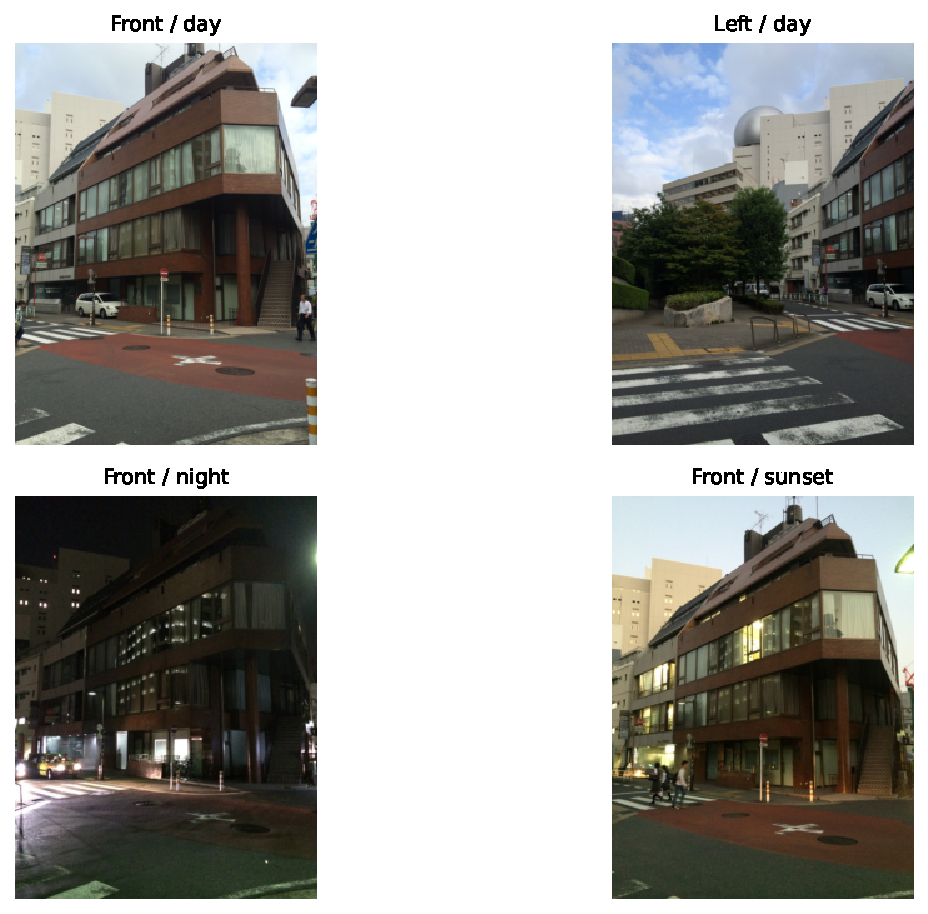
\includegraphics[width=.92\textwidth]{evidence/tokyo_09.pdf}
\caption{All retained photographs for tokyo\_009.}\label{fig:tokyo-scene-9}\end{figure}

\begin{table}[H]\centering\small
\caption{All main-method decisions for tokyo\_009.}\label{tab:tokyo-site-9}
\begin{tabular}{llrlr}\toprule
Protocol & Method & R & Decision & Selected inliers \\
\midrule
D--D & SIFT & 1 & correct & 100 \\
D--D & SP+LG & 1 & correct & 186 \\
D--D & Global & 1 & ranking only & -- \\
D--D & Full & 1 & correct & 186 \\
D--N & SIFT & 1 & correct & 12 \\
D--N & SP+LG & 1 & correct & 190 \\
D--N & Global & 1 & ranking only & -- \\
D--N & Full & 1 & correct & 190 \\
N--D & SIFT & 1 & correct & 13 \\
N--D & SP+LG & 1 & correct & 189 \\
N--D & Global & 1 & ranking only & -- \\
N--D & Full & 1 & correct & 189 \\
D--S & SIFT & 1 & correct & 76 \\
D--S & SP+LG & 1 & correct & 307 \\
D--S & Global & 1 & ranking only & -- \\
D--S & Full & 1 & correct & 307 \\
\bottomrule\end{tabular}\end{table}


Across these four protocols, SIFT correctly verifies 4, exhaustive SP+LG 4, and the full hierarchy 4 of the four queries. The full hierarchy makes 0 wrong-place acceptances and 0 rejections. These counts separate a missing anchor from an incorrectly accepted identity; the latter is the more direct location-association failure.

For this site, the full-pipeline changed-direction daytime query is correctly verified, while its front-facing day-to-night query is correctly verified. This paired observation should be read with the photographs and the rank column. It does not identify the causal effect of illumination alone, because overlap and view direction also change between the protocols. No corner-error or metric-pose value is inferred from a correct place label.

\section{Site tokyo\_010}

This site contributes four real photographs and four labelled retrieval queries. Each protocol uses one of the photographs as its query and the condition-specific 24-site gallery defined in the frozen benchmark. Reusing a site across protocols produces paired condition observations, not four new geographic locations.

\begin{figure}[H]\centering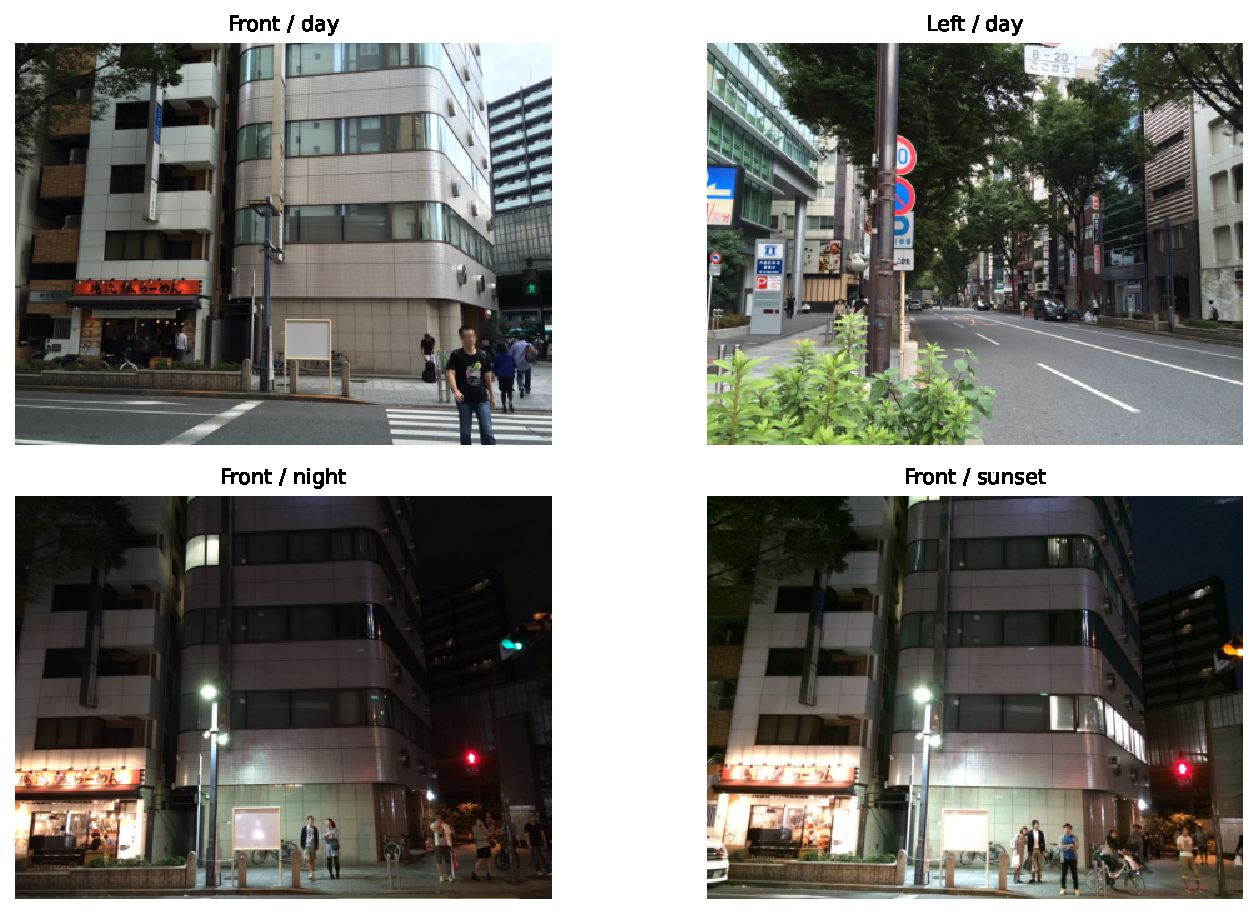
\includegraphics[width=.92\textwidth]{evidence/tokyo_10.pdf}
\caption{All retained photographs for tokyo\_010.}\label{fig:tokyo-scene-10}\end{figure}

\begin{table}[H]\centering\small
\caption{All main-method decisions for tokyo\_010.}\label{tab:tokyo-site-10}
\begin{tabular}{llrlr}\toprule
Protocol & Method & R & Decision & Selected inliers \\
\midrule
D--D & SIFT & 2 & rejected & 0 \\
D--D & SP+LG & 1 & rejected & 0 \\
D--D & Global & 18 & ranking only & -- \\
D--D & Full & 18 & rejected & 0 \\
D--N & SIFT & 2 & rejected & 0 \\
D--N & SP+LG & 1 & correct & 198 \\
D--N & Global & 1 & ranking only & -- \\
D--N & Full & 1 & correct & 198 \\
N--D & SIFT & 1 & rejected & 0 \\
N--D & SP+LG & 1 & correct & 185 \\
N--D & Global & 1 & ranking only & -- \\
N--D & Full & 1 & correct & 185 \\
D--S & SIFT & 2 & rejected & 0 \\
D--S & SP+LG & 1 & correct & 207 \\
D--S & Global & 1 & ranking only & -- \\
D--S & Full & 1 & correct & 207 \\
\bottomrule\end{tabular}\end{table}


Across these four protocols, SIFT correctly verifies 0, exhaustive SP+LG 3, and the full hierarchy 3 of the four queries. The full hierarchy makes 0 wrong-place acceptances and 1 rejection. These counts separate a missing anchor from an incorrectly accepted identity; the latter is the more direct location-association failure.

For this site, the full-pipeline changed-direction daytime query is rejected, while its front-facing day-to-night query is correctly verified. This paired observation should be read with the photographs and the rank column. It does not identify the causal effect of illumination alone, because overlap and view direction also change between the protocols. No corner-error or metric-pose value is inferred from a correct place label.

\section{Site tokyo\_011}

This site contributes four real photographs and four labelled retrieval queries. Each protocol uses one of the photographs as its query and the condition-specific 24-site gallery defined in the frozen benchmark. Reusing a site across protocols produces paired condition observations, not four new geographic locations.

\begin{figure}[H]\centering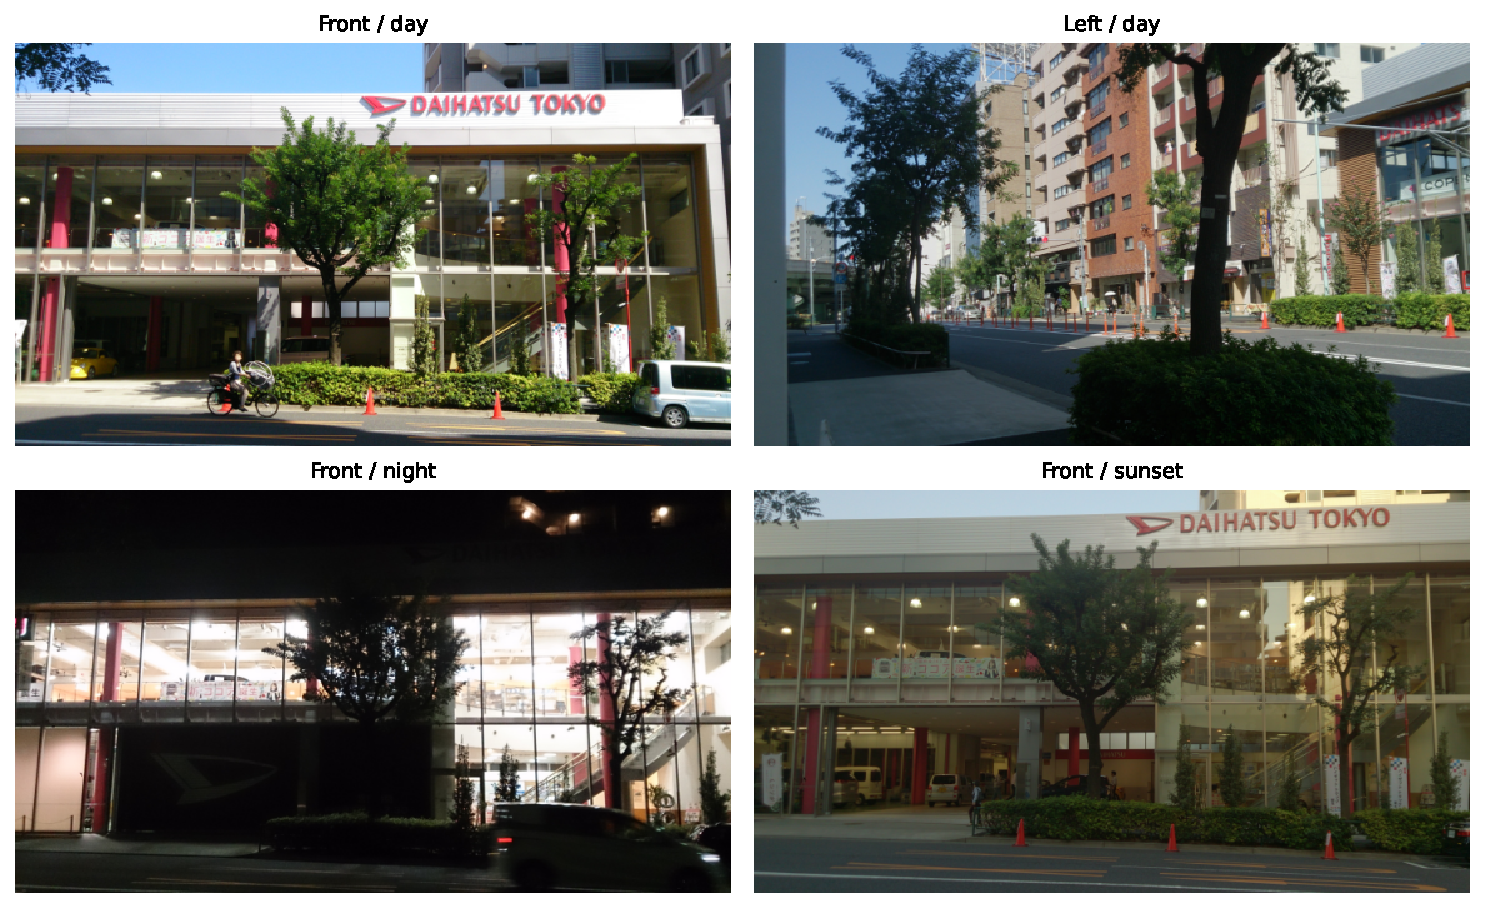
\includegraphics[width=.92\textwidth]{evidence/tokyo_11.pdf}
\caption{All retained photographs for tokyo\_011.}\label{fig:tokyo-scene-11}\end{figure}

\begin{table}[H]\centering\small
\caption{All main-method decisions for tokyo\_011.}\label{tab:tokyo-site-11}
\begin{tabular}{llrlr}\toprule
Protocol & Method & R & Decision & Selected inliers \\
\midrule
D--D & SIFT & 14 & rejected & 0 \\
D--D & SP+LG & 18 & wrong & 18 \\
D--D & Global & 7 & ranking only & -- \\
D--D & Full & 7 & rejected & 0 \\
D--N & SIFT & 16 & rejected & 0 \\
D--N & SP+LG & 1 & correct & 141 \\
D--N & Global & 1 & ranking only & -- \\
D--N & Full & 1 & correct & 141 \\
N--D & SIFT & 17 & rejected & 0 \\
N--D & SP+LG & 1 & correct & 138 \\
N--D & Global & 1 & ranking only & -- \\
N--D & Full & 1 & correct & 138 \\
D--S & SIFT & 3 & rejected & 0 \\
D--S & SP+LG & 1 & correct & 128 \\
D--S & Global & 1 & ranking only & -- \\
D--S & Full & 1 & correct & 128 \\
\bottomrule\end{tabular}\end{table}


Across these four protocols, SIFT correctly verifies 0, exhaustive SP+LG 3, and the full hierarchy 3 of the four queries. The full hierarchy makes 0 wrong-place acceptances and 1 rejection. These counts separate a missing anchor from an incorrectly accepted identity; the latter is the more direct location-association failure.

For this site, the full-pipeline changed-direction daytime query is rejected, while its front-facing day-to-night query is correctly verified. This paired observation should be read with the photographs and the rank column. It does not identify the causal effect of illumination alone, because overlap and view direction also change between the protocols. No corner-error or metric-pose value is inferred from a correct place label.

\section{Site tokyo\_012}

This site contributes four real photographs and four labelled retrieval queries. Each protocol uses one of the photographs as its query and the condition-specific 24-site gallery defined in the frozen benchmark. Reusing a site across protocols produces paired condition observations, not four new geographic locations.

\begin{figure}[H]\centering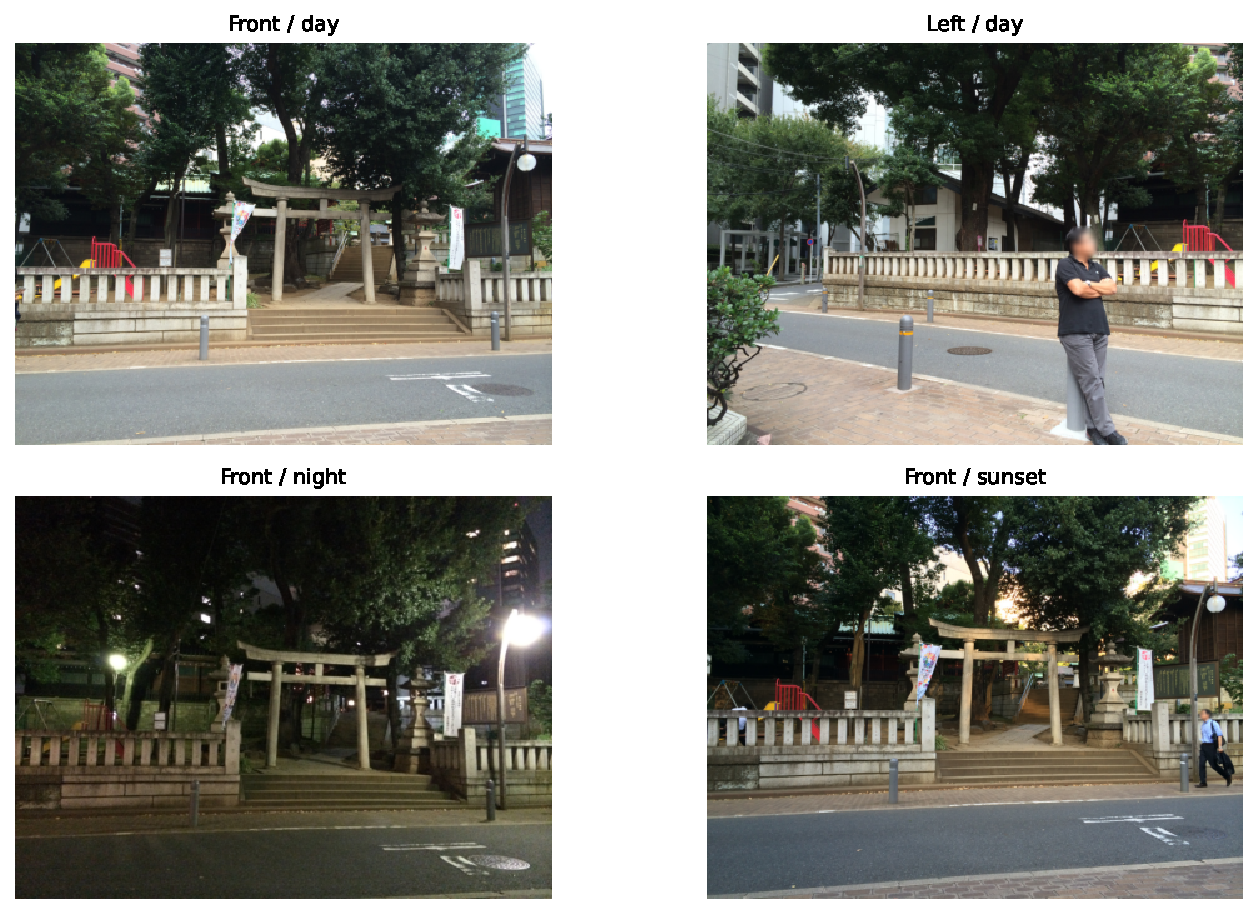
\includegraphics[width=.92\textwidth]{evidence/tokyo_12.pdf}
\caption{All retained photographs for tokyo\_012.}\label{fig:tokyo-scene-12}\end{figure}

\begin{table}[H]\centering\small
\caption{All main-method decisions for tokyo\_012.}\label{tab:tokyo-site-12}
\begin{tabular}{llrlr}\toprule
Protocol & Method & R & Decision & Selected inliers \\
\midrule
D--D & SIFT & 1 & correct & 15 \\
D--D & SP+LG & 1 & correct & 56 \\
D--D & Global & 1 & ranking only & -- \\
D--D & Full & 1 & correct & 56 \\
D--N & SIFT & 1 & correct & 22 \\
D--N & SP+LG & 1 & correct & 231 \\
D--N & Global & 1 & ranking only & -- \\
D--N & Full & 1 & correct & 231 \\
N--D & SIFT & 1 & correct & 18 \\
N--D & SP+LG & 1 & correct & 234 \\
N--D & Global & 1 & ranking only & -- \\
N--D & Full & 1 & correct & 234 \\
D--S & SIFT & 1 & correct & 113 \\
D--S & SP+LG & 1 & correct & 316 \\
D--S & Global & 1 & ranking only & -- \\
D--S & Full & 1 & correct & 316 \\
\bottomrule\end{tabular}\end{table}


Across these four protocols, SIFT correctly verifies 4, exhaustive SP+LG 4, and the full hierarchy 4 of the four queries. The full hierarchy makes 0 wrong-place acceptances and 0 rejections. These counts separate a missing anchor from an incorrectly accepted identity; the latter is the more direct location-association failure.

For this site, the full-pipeline changed-direction daytime query is correctly verified, while its front-facing day-to-night query is correctly verified. This paired observation should be read with the photographs and the rank column. It does not identify the causal effect of illumination alone, because overlap and view direction also change between the protocols. No corner-error or metric-pose value is inferred from a correct place label.

\section{Site tokyo\_013}

This site contributes four real photographs and four labelled retrieval queries. Each protocol uses one of the photographs as its query and the condition-specific 24-site gallery defined in the frozen benchmark. Reusing a site across protocols produces paired condition observations, not four new geographic locations.

\begin{figure}[H]\centering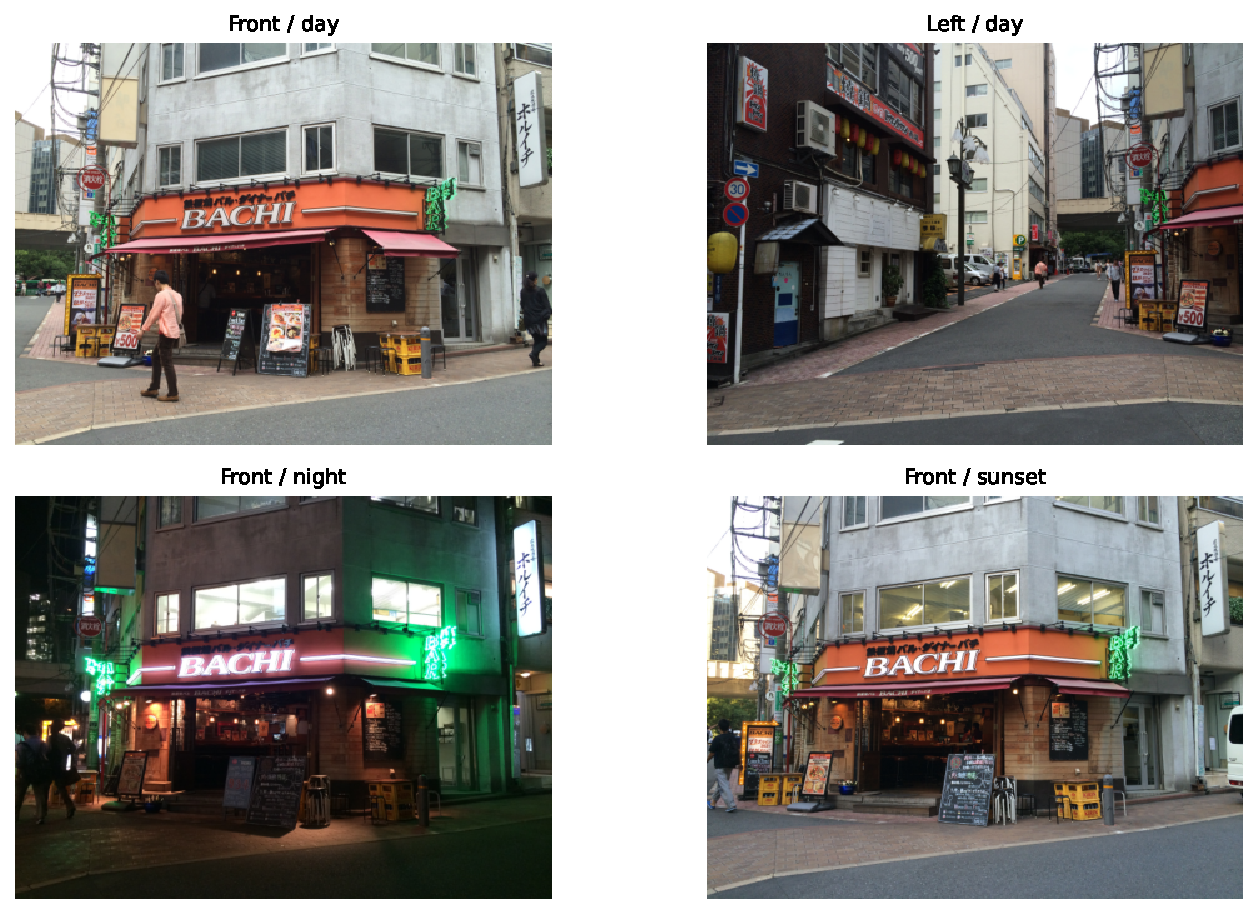
\includegraphics[width=.92\textwidth]{evidence/tokyo_13.pdf}
\caption{All retained photographs for tokyo\_013.}\label{fig:tokyo-scene-13}\end{figure}

\begin{table}[H]\centering\small
\caption{All main-method decisions for tokyo\_013.}\label{tab:tokyo-site-13}
\begin{tabular}{llrlr}\toprule
Protocol & Method & R & Decision & Selected inliers \\
\midrule
D--D & SIFT & 1 & correct & 44 \\
D--D & SP+LG & 1 & correct & 70 \\
D--D & Global & 11 & ranking only & -- \\
D--D & Full & 11 & rejected & 0 \\
D--N & SIFT & 1 & rejected & 0 \\
D--N & SP+LG & 1 & correct & 170 \\
D--N & Global & 1 & ranking only & -- \\
D--N & Full & 1 & correct & 170 \\
N--D & SIFT & 1 & rejected & 0 \\
N--D & SP+LG & 1 & correct & 167 \\
N--D & Global & 1 & ranking only & -- \\
N--D & Full & 1 & correct & 167 \\
D--S & SIFT & 1 & correct & 119 \\
D--S & SP+LG & 1 & correct & 255 \\
D--S & Global & 1 & ranking only & -- \\
D--S & Full & 1 & correct & 255 \\
\bottomrule\end{tabular}\end{table}


Across these four protocols, SIFT correctly verifies 2, exhaustive SP+LG 4, and the full hierarchy 3 of the four queries. The full hierarchy makes 0 wrong-place acceptances and 1 rejection. These counts separate a missing anchor from an incorrectly accepted identity; the latter is the more direct location-association failure.

For this site, the full-pipeline changed-direction daytime query is rejected, while its front-facing day-to-night query is correctly verified. This paired observation should be read with the photographs and the rank column. It does not identify the causal effect of illumination alone, because overlap and view direction also change between the protocols. No corner-error or metric-pose value is inferred from a correct place label.

\section{Site tokyo\_014}

This site contributes four real photographs and four labelled retrieval queries. Each protocol uses one of the photographs as its query and the condition-specific 24-site gallery defined in the frozen benchmark. Reusing a site across protocols produces paired condition observations, not four new geographic locations.

\begin{figure}[H]\centering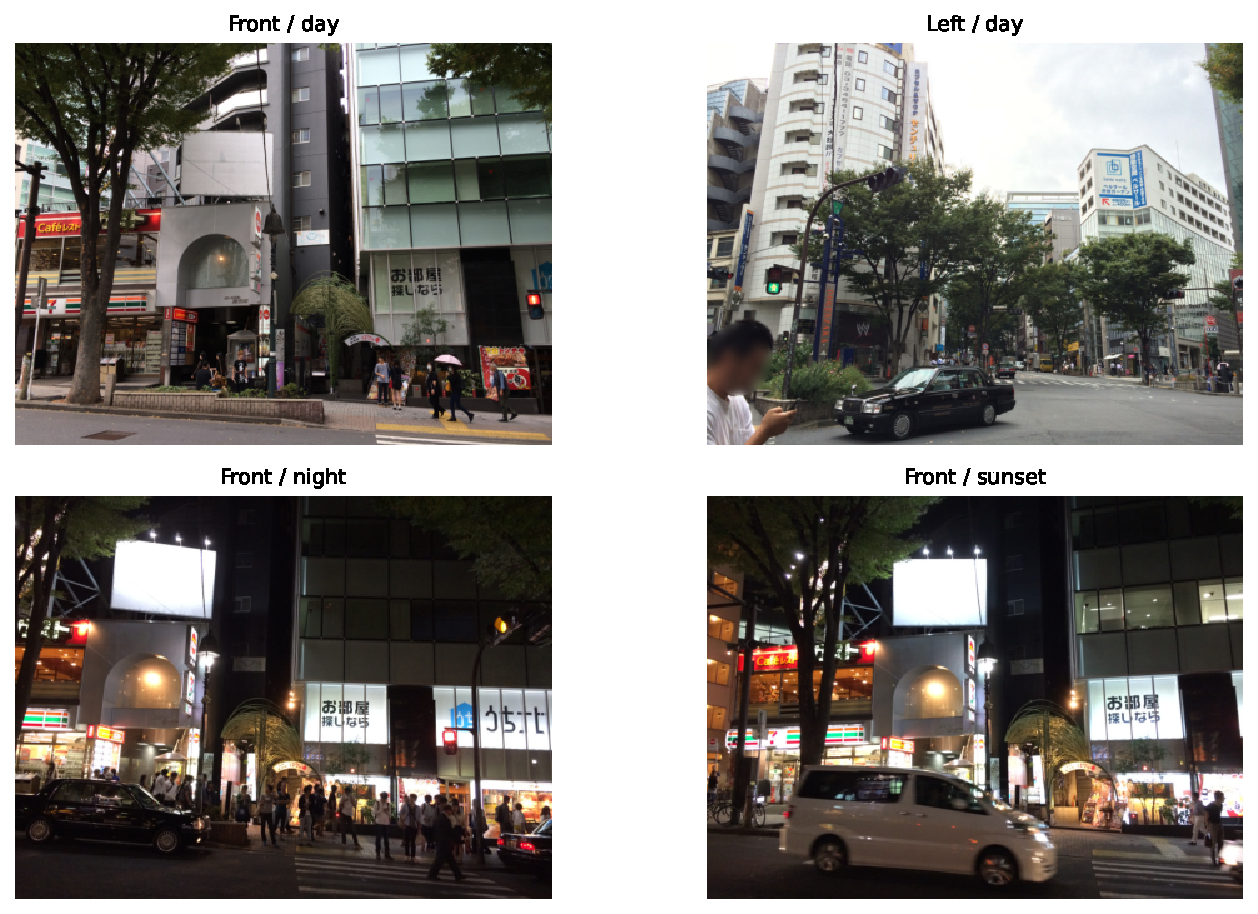
\includegraphics[width=.92\textwidth]{evidence/tokyo_14.pdf}
\caption{All retained photographs for tokyo\_014.}\label{fig:tokyo-scene-14}\end{figure}

\begin{table}[H]\centering\small
\caption{All main-method decisions for tokyo\_014.}\label{tab:tokyo-site-14}
\begin{tabular}{llrlr}\toprule
Protocol & Method & R & Decision & Selected inliers \\
\midrule
D--D & SIFT & 18 & rejected & 0 \\
D--D & SP+LG & 16 & wrong & 17 \\
D--D & Global & 18 & ranking only & -- \\
D--D & Full & 18 & rejected & 0 \\
D--N & SIFT & 2 & rejected & 0 \\
D--N & SP+LG & 1 & correct & 125 \\
D--N & Global & 1 & ranking only & -- \\
D--N & Full & 1 & correct & 125 \\
N--D & SIFT & 2 & rejected & 0 \\
N--D & SP+LG & 1 & correct & 140 \\
N--D & Global & 1 & ranking only & -- \\
N--D & Full & 1 & correct & 140 \\
D--S & SIFT & 1 & rejected & 0 \\
D--S & SP+LG & 1 & correct & 173 \\
D--S & Global & 1 & ranking only & -- \\
D--S & Full & 1 & correct & 173 \\
\bottomrule\end{tabular}\end{table}


Across these four protocols, SIFT correctly verifies 0, exhaustive SP+LG 3, and the full hierarchy 3 of the four queries. The full hierarchy makes 0 wrong-place acceptances and 1 rejection. These counts separate a missing anchor from an incorrectly accepted identity; the latter is the more direct location-association failure.

For this site, the full-pipeline changed-direction daytime query is rejected, while its front-facing day-to-night query is correctly verified. This paired observation should be read with the photographs and the rank column. It does not identify the causal effect of illumination alone, because overlap and view direction also change between the protocols. No corner-error or metric-pose value is inferred from a correct place label.

\section{Site tokyo\_015}

This site contributes four real photographs and four labelled retrieval queries. Each protocol uses one of the photographs as its query and the condition-specific 24-site gallery defined in the frozen benchmark. Reusing a site across protocols produces paired condition observations, not four new geographic locations.

\begin{figure}[H]\centering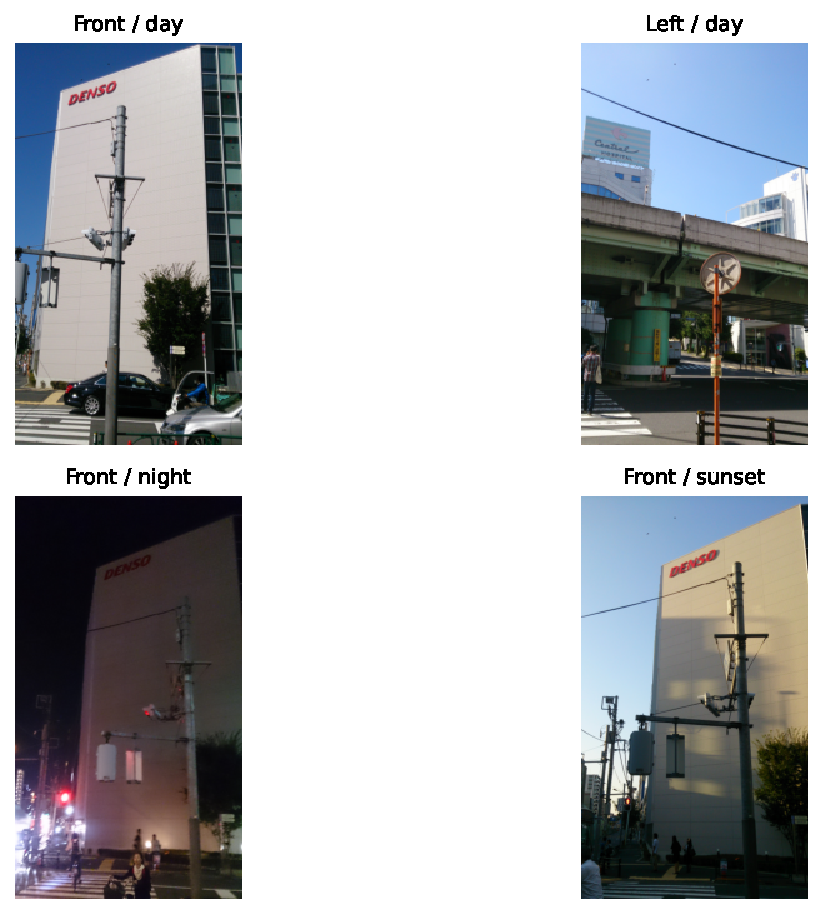
\includegraphics[width=.92\textwidth]{evidence/tokyo_15.pdf}
\caption{All retained photographs for tokyo\_015.}\label{fig:tokyo-scene-15}\end{figure}

\begin{table}[H]\centering\small
\caption{All main-method decisions for tokyo\_015.}\label{tab:tokyo-site-15}
\begin{tabular}{llrlr}\toprule
Protocol & Method & R & Decision & Selected inliers \\
\midrule
D--D & SIFT & 8 & rejected & 0 \\
D--D & SP+LG & 17 & wrong & 15 \\
D--D & Global & 5 & ranking only & -- \\
D--D & Full & 5 & wrong & 15 \\
D--N & SIFT & 1 & rejected & 0 \\
D--N & SP+LG & 1 & correct & 39 \\
D--N & Global & 1 & ranking only & -- \\
D--N & Full & 1 & correct & 39 \\
N--D & SIFT & 8 & rejected & 0 \\
N--D & SP+LG & 1 & correct & 47 \\
N--D & Global & 1 & ranking only & -- \\
N--D & Full & 1 & correct & 47 \\
D--S & SIFT & 1 & rejected & 0 \\
D--S & SP+LG & 1 & correct & 69 \\
D--S & Global & 1 & ranking only & -- \\
D--S & Full & 1 & correct & 69 \\
\bottomrule\end{tabular}\end{table}


Across these four protocols, SIFT correctly verifies 0, exhaustive SP+LG 3, and the full hierarchy 3 of the four queries. The full hierarchy makes 1 wrong-place acceptance and 0 rejections. These counts separate a missing anchor from an incorrectly accepted identity; the latter is the more direct location-association failure.

For this site, the full-pipeline changed-direction daytime query is accepted at the wrong place, while its front-facing day-to-night query is correctly verified. This paired observation should be read with the photographs and the rank column. It does not identify the causal effect of illumination alone, because overlap and view direction also change between the protocols. No corner-error or metric-pose value is inferred from a correct place label.

\section{Site tokyo\_016}

This site contributes four real photographs and four labelled retrieval queries. Each protocol uses one of the photographs as its query and the condition-specific 24-site gallery defined in the frozen benchmark. Reusing a site across protocols produces paired condition observations, not four new geographic locations.

\begin{figure}[H]\centering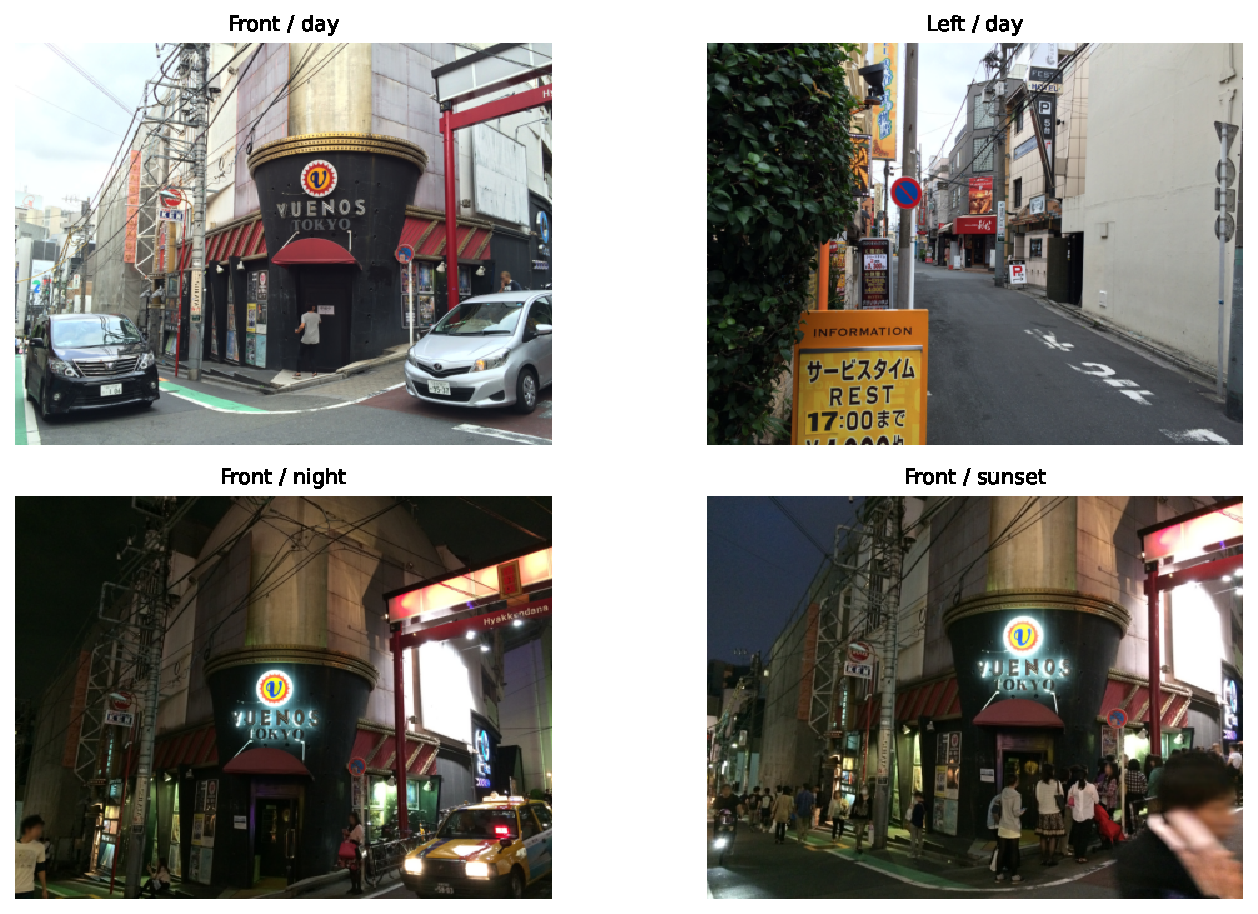
\includegraphics[width=.92\textwidth]{evidence/tokyo_16.pdf}
\caption{All retained photographs for tokyo\_016.}\label{fig:tokyo-scene-16}\end{figure}

\begin{table}[H]\centering\small
\caption{All main-method decisions for tokyo\_016.}\label{tab:tokyo-site-16}
\begin{tabular}{llrlr}\toprule
Protocol & Method & R & Decision & Selected inliers \\
\midrule
D--D & SIFT & 1 & rejected & 0 \\
D--D & SP+LG & 6 & rejected & 0 \\
D--D & Global & 4 & ranking only & -- \\
D--D & Full & 4 & rejected & 0 \\
D--N & SIFT & 1 & rejected & 0 \\
D--N & SP+LG & 1 & correct & 167 \\
D--N & Global & 1 & ranking only & -- \\
D--N & Full & 1 & correct & 167 \\
N--D & SIFT & 1 & rejected & 0 \\
N--D & SP+LG & 1 & correct & 167 \\
N--D & Global & 1 & ranking only & -- \\
N--D & Full & 1 & correct & 167 \\
D--S & SIFT & 2 & rejected & 0 \\
D--S & SP+LG & 1 & correct & 110 \\
D--S & Global & 1 & ranking only & -- \\
D--S & Full & 1 & correct & 110 \\
\bottomrule\end{tabular}\end{table}


Across these four protocols, SIFT correctly verifies 0, exhaustive SP+LG 3, and the full hierarchy 3 of the four queries. The full hierarchy makes 0 wrong-place acceptances and 1 rejection. These counts separate a missing anchor from an incorrectly accepted identity; the latter is the more direct location-association failure.

For this site, the full-pipeline changed-direction daytime query is rejected, while its front-facing day-to-night query is correctly verified. This paired observation should be read with the photographs and the rank column. It does not identify the causal effect of illumination alone, because overlap and view direction also change between the protocols. No corner-error or metric-pose value is inferred from a correct place label.

\section{Site tokyo\_017}

This site contributes four real photographs and four labelled retrieval queries. Each protocol uses one of the photographs as its query and the condition-specific 24-site gallery defined in the frozen benchmark. Reusing a site across protocols produces paired condition observations, not four new geographic locations.

\begin{figure}[H]\centering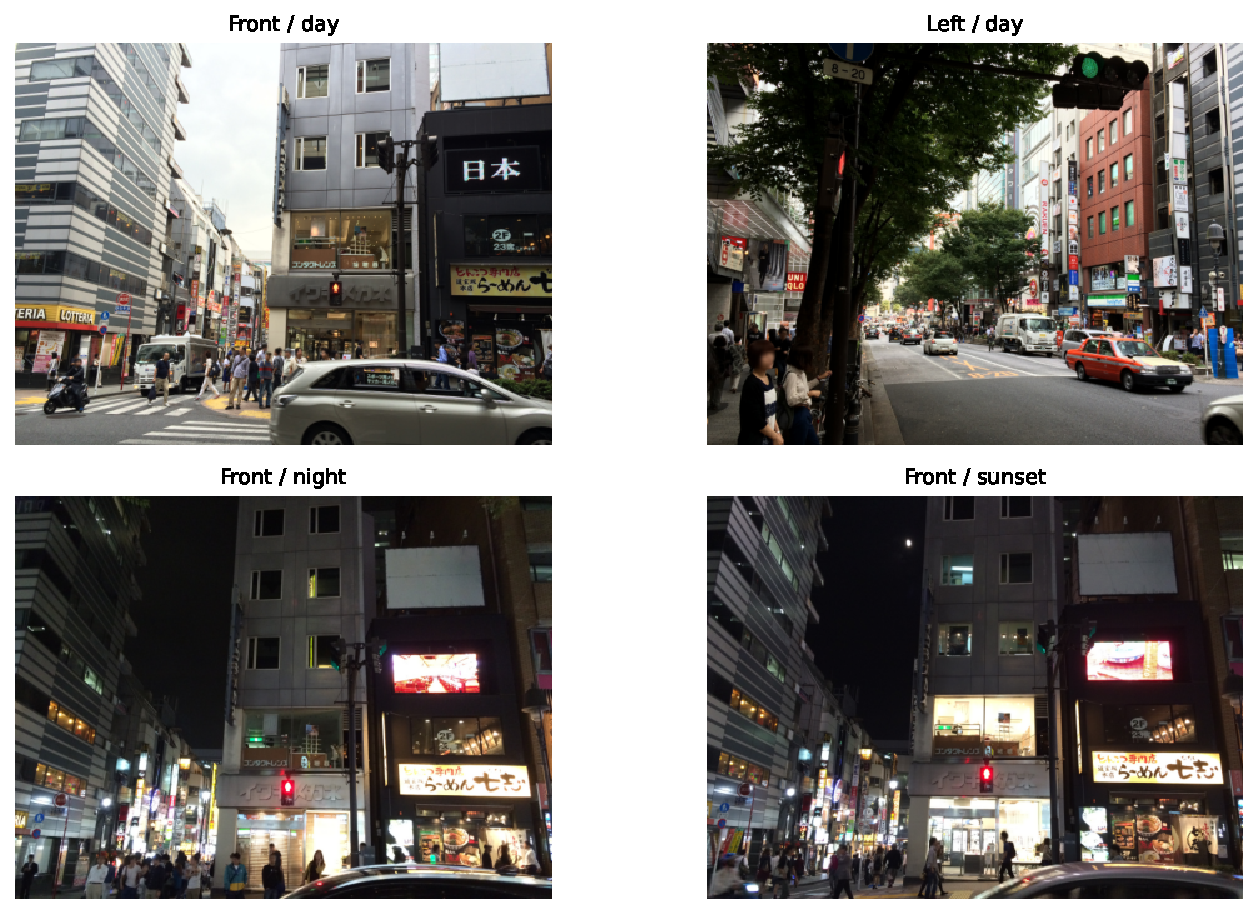
\includegraphics[width=.92\textwidth]{evidence/tokyo_17.pdf}
\caption{All retained photographs for tokyo\_017.}\label{fig:tokyo-scene-17}\end{figure}

\begin{table}[H]\centering\small
\caption{All main-method decisions for tokyo\_017.}\label{tab:tokyo-site-17}
\begin{tabular}{llrlr}\toprule
Protocol & Method & R & Decision & Selected inliers \\
\midrule
D--D & SIFT & 21 & rejected & 0 \\
D--D & SP+LG & 2 & rejected & 0 \\
D--D & Global & 8 & ranking only & -- \\
D--D & Full & 8 & rejected & 0 \\
D--N & SIFT & 2 & rejected & 0 \\
D--N & SP+LG & 1 & correct & 164 \\
D--N & Global & 1 & ranking only & -- \\
D--N & Full & 1 & correct & 164 \\
N--D & SIFT & 2 & rejected & 0 \\
N--D & SP+LG & 1 & correct & 164 \\
N--D & Global & 1 & ranking only & -- \\
N--D & Full & 1 & correct & 164 \\
D--S & SIFT & 1 & rejected & 0 \\
D--S & SP+LG & 1 & correct & 113 \\
D--S & Global & 1 & ranking only & -- \\
D--S & Full & 1 & correct & 113 \\
\bottomrule\end{tabular}\end{table}


Across these four protocols, SIFT correctly verifies 0, exhaustive SP+LG 3, and the full hierarchy 3 of the four queries. The full hierarchy makes 0 wrong-place acceptances and 1 rejection. These counts separate a missing anchor from an incorrectly accepted identity; the latter is the more direct location-association failure.

For this site, the full-pipeline changed-direction daytime query is rejected, while its front-facing day-to-night query is correctly verified. This paired observation should be read with the photographs and the rank column. It does not identify the causal effect of illumination alone, because overlap and view direction also change between the protocols. No corner-error or metric-pose value is inferred from a correct place label.

\section{Site tokyo\_018}

This site contributes four real photographs and four labelled retrieval queries. Each protocol uses one of the photographs as its query and the condition-specific 24-site gallery defined in the frozen benchmark. Reusing a site across protocols produces paired condition observations, not four new geographic locations.

\begin{figure}[H]\centering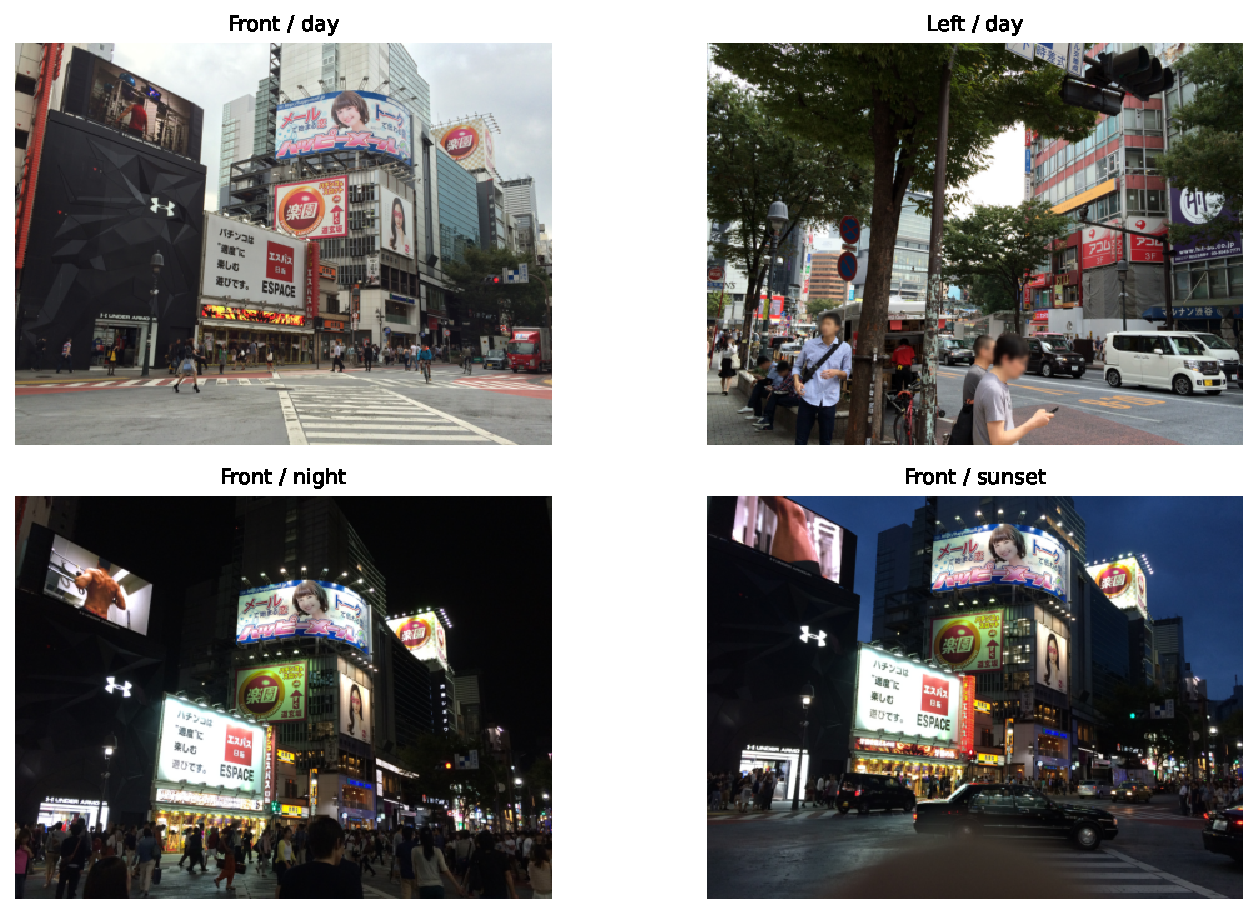
\includegraphics[width=.92\textwidth]{evidence/tokyo_18.pdf}
\caption{All retained photographs for tokyo\_018.}\label{fig:tokyo-scene-18}\end{figure}

\begin{table}[H]\centering\small
\caption{All main-method decisions for tokyo\_018.}\label{tab:tokyo-site-18}
\begin{tabular}{llrlr}\toprule
Protocol & Method & R & Decision & Selected inliers \\
\midrule
D--D & SIFT & 20 & rejected & 0 \\
D--D & SP+LG & 16 & rejected & 0 \\
D--D & Global & 2 & ranking only & -- \\
D--D & Full & 1 & rejected & 0 \\
D--N & SIFT & 1 & correct & 34 \\
D--N & SP+LG & 1 & correct & 152 \\
D--N & Global & 1 & ranking only & -- \\
D--N & Full & 1 & correct & 152 \\
N--D & SIFT & 1 & correct & 33 \\
N--D & SP+LG & 1 & correct & 162 \\
N--D & Global & 1 & ranking only & -- \\
N--D & Full & 1 & correct & 162 \\
D--S & SIFT & 1 & correct & 33 \\
D--S & SP+LG & 1 & correct & 201 \\
D--S & Global & 1 & ranking only & -- \\
D--S & Full & 1 & correct & 201 \\
\bottomrule\end{tabular}\end{table}


Across these four protocols, SIFT correctly verifies 3, exhaustive SP+LG 3, and the full hierarchy 3 of the four queries. The full hierarchy makes 0 wrong-place acceptances and 1 rejection. These counts separate a missing anchor from an incorrectly accepted identity; the latter is the more direct location-association failure.

For this site, the full-pipeline changed-direction daytime query is rejected, while its front-facing day-to-night query is correctly verified. This paired observation should be read with the photographs and the rank column. It does not identify the causal effect of illumination alone, because overlap and view direction also change between the protocols. No corner-error or metric-pose value is inferred from a correct place label.

\section{Site tokyo\_019}

This site contributes four real photographs and four labelled retrieval queries. Each protocol uses one of the photographs as its query and the condition-specific 24-site gallery defined in the frozen benchmark. Reusing a site across protocols produces paired condition observations, not four new geographic locations.

\begin{figure}[H]\centering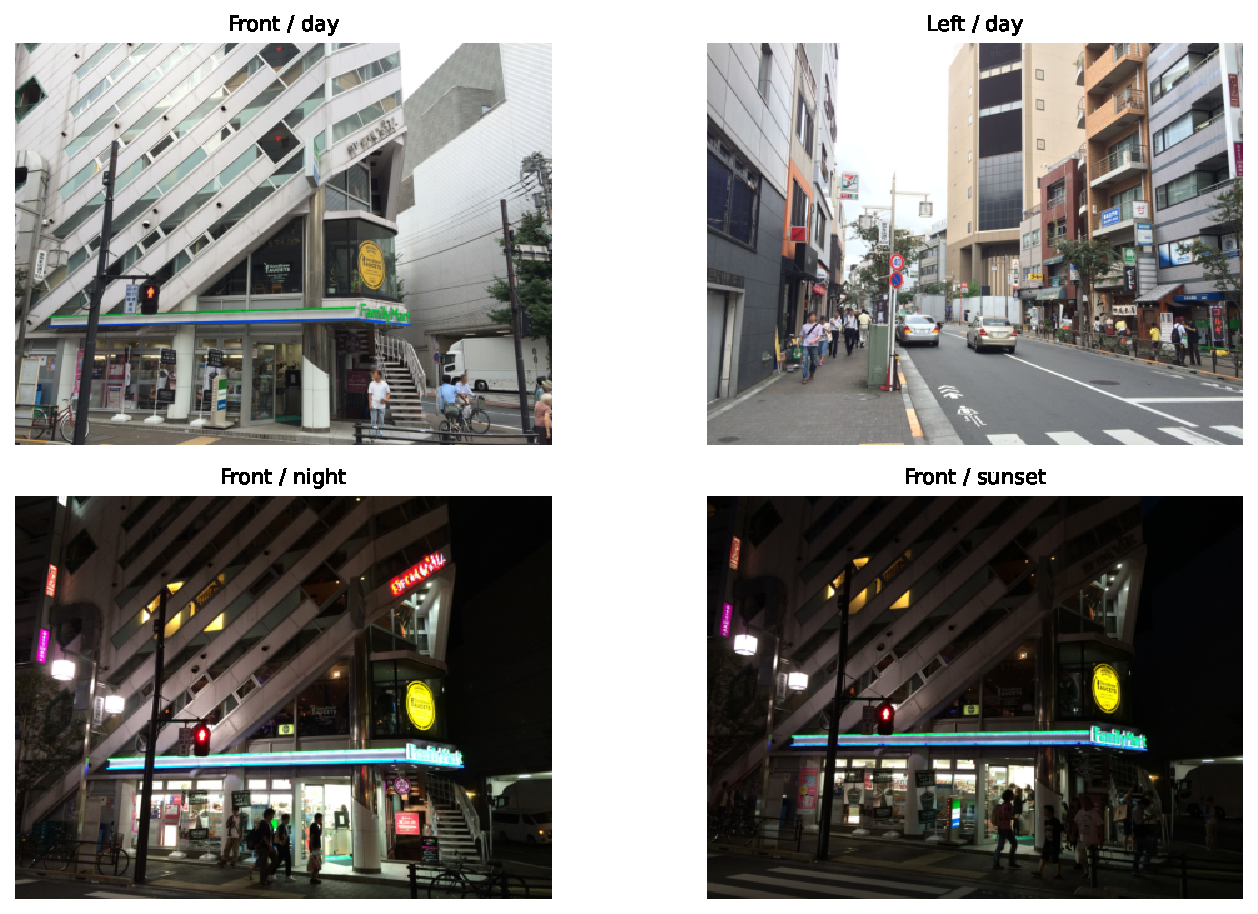
\includegraphics[width=.92\textwidth]{evidence/tokyo_19.pdf}
\caption{All retained photographs for tokyo\_019.}\label{fig:tokyo-scene-19}\end{figure}

\begin{table}[H]\centering\small
\caption{All main-method decisions for tokyo\_019.}\label{tab:tokyo-site-19}
\begin{tabular}{llrlr}\toprule
Protocol & Method & R & Decision & Selected inliers \\
\midrule
D--D & SIFT & 9 & rejected & 0 \\
D--D & SP+LG & 11 & rejected & 0 \\
D--D & Global & 13 & ranking only & -- \\
D--D & Full & 13 & rejected & 0 \\
D--N & SIFT & 1 & rejected & 0 \\
D--N & SP+LG & 1 & correct & 178 \\
D--N & Global & 1 & ranking only & -- \\
D--N & Full & 1 & correct & 178 \\
N--D & SIFT & 6 & rejected & 0 \\
N--D & SP+LG & 1 & correct & 180 \\
N--D & Global & 1 & ranking only & -- \\
N--D & Full & 1 & correct & 180 \\
D--S & SIFT & 6 & rejected & 0 \\
D--S & SP+LG & 1 & correct & 171 \\
D--S & Global & 1 & ranking only & -- \\
D--S & Full & 1 & correct & 171 \\
\bottomrule\end{tabular}\end{table}


Across these four protocols, SIFT correctly verifies 0, exhaustive SP+LG 3, and the full hierarchy 3 of the four queries. The full hierarchy makes 0 wrong-place acceptances and 1 rejection. These counts separate a missing anchor from an incorrectly accepted identity; the latter is the more direct location-association failure.

For this site, the full-pipeline changed-direction daytime query is rejected, while its front-facing day-to-night query is correctly verified. This paired observation should be read with the photographs and the rank column. It does not identify the causal effect of illumination alone, because overlap and view direction also change between the protocols. No corner-error or metric-pose value is inferred from a correct place label.

\section{Site tokyo\_020}

This site contributes four real photographs and four labelled retrieval queries. Each protocol uses one of the photographs as its query and the condition-specific 24-site gallery defined in the frozen benchmark. Reusing a site across protocols produces paired condition observations, not four new geographic locations.

\begin{figure}[H]\centering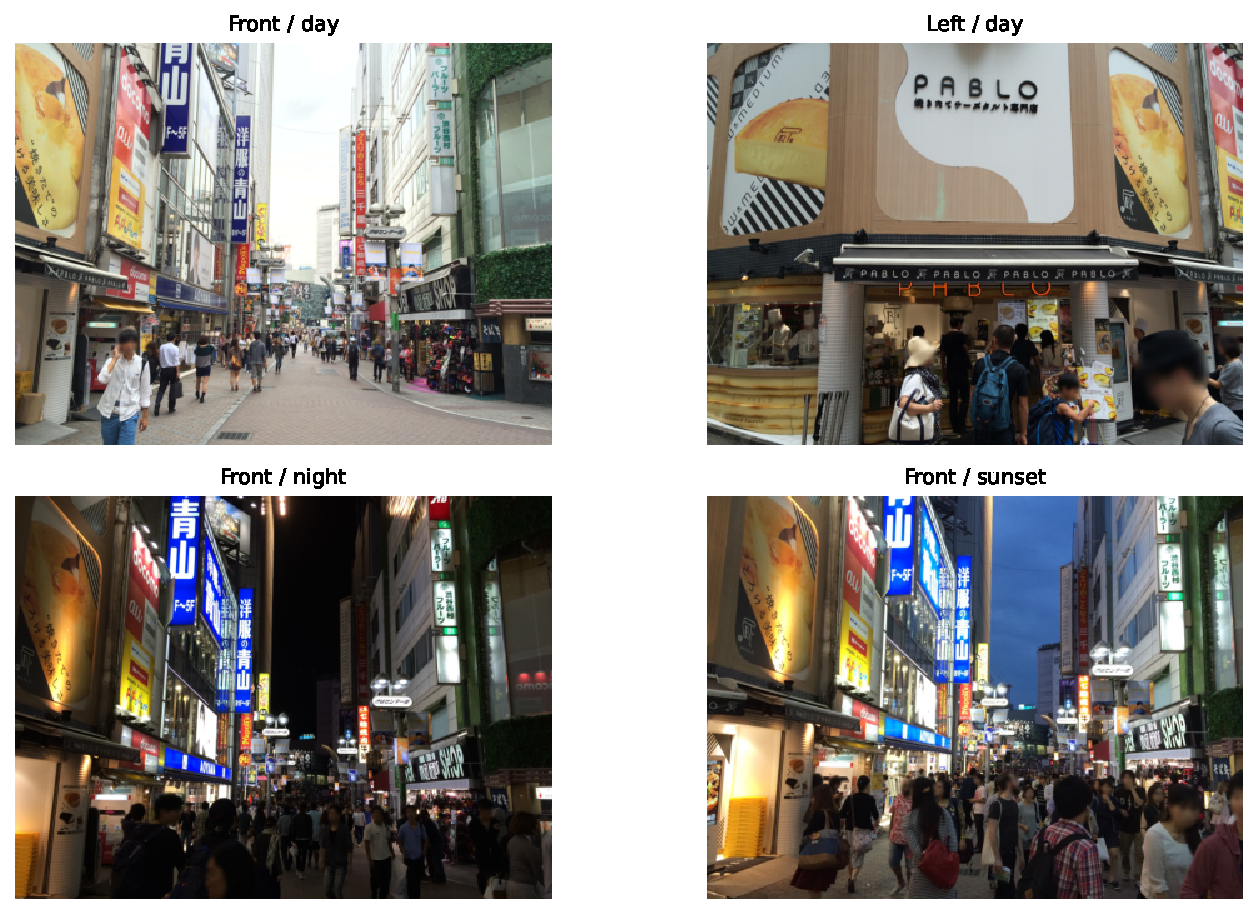
\includegraphics[width=.92\textwidth]{evidence/tokyo_20.pdf}
\caption{All retained photographs for tokyo\_020.}\label{fig:tokyo-scene-20}\end{figure}

\begin{table}[H]\centering\small
\caption{All main-method decisions for tokyo\_020.}\label{tab:tokyo-site-20}
\begin{tabular}{llrlr}\toprule
Protocol & Method & R & Decision & Selected inliers \\
\midrule
D--D & SIFT & 4 & rejected & 0 \\
D--D & SP+LG & 1 & correct & 44 \\
D--D & Global & 4 & ranking only & -- \\
D--D & Full & 4 & rejected & 0 \\
D--N & SIFT & 1 & correct & 23 \\
D--N & SP+LG & 1 & correct & 139 \\
D--N & Global & 1 & ranking only & -- \\
D--N & Full & 1 & correct & 139 \\
N--D & SIFT & 1 & correct & 22 \\
N--D & SP+LG & 1 & correct & 140 \\
N--D & Global & 1 & ranking only & -- \\
N--D & Full & 1 & correct & 140 \\
D--S & SIFT & 1 & correct & 25 \\
D--S & SP+LG & 1 & correct & 140 \\
D--S & Global & 1 & ranking only & -- \\
D--S & Full & 1 & correct & 140 \\
\bottomrule\end{tabular}\end{table}


Across these four protocols, SIFT correctly verifies 3, exhaustive SP+LG 4, and the full hierarchy 3 of the four queries. The full hierarchy makes 0 wrong-place acceptances and 1 rejection. These counts separate a missing anchor from an incorrectly accepted identity; the latter is the more direct location-association failure.

For this site, the full-pipeline changed-direction daytime query is rejected, while its front-facing day-to-night query is correctly verified. This paired observation should be read with the photographs and the rank column. It does not identify the causal effect of illumination alone, because overlap and view direction also change between the protocols. No corner-error or metric-pose value is inferred from a correct place label.

\section{Site tokyo\_021}

This site contributes four real photographs and four labelled retrieval queries. Each protocol uses one of the photographs as its query and the condition-specific 24-site gallery defined in the frozen benchmark. Reusing a site across protocols produces paired condition observations, not four new geographic locations.

\begin{figure}[H]\centering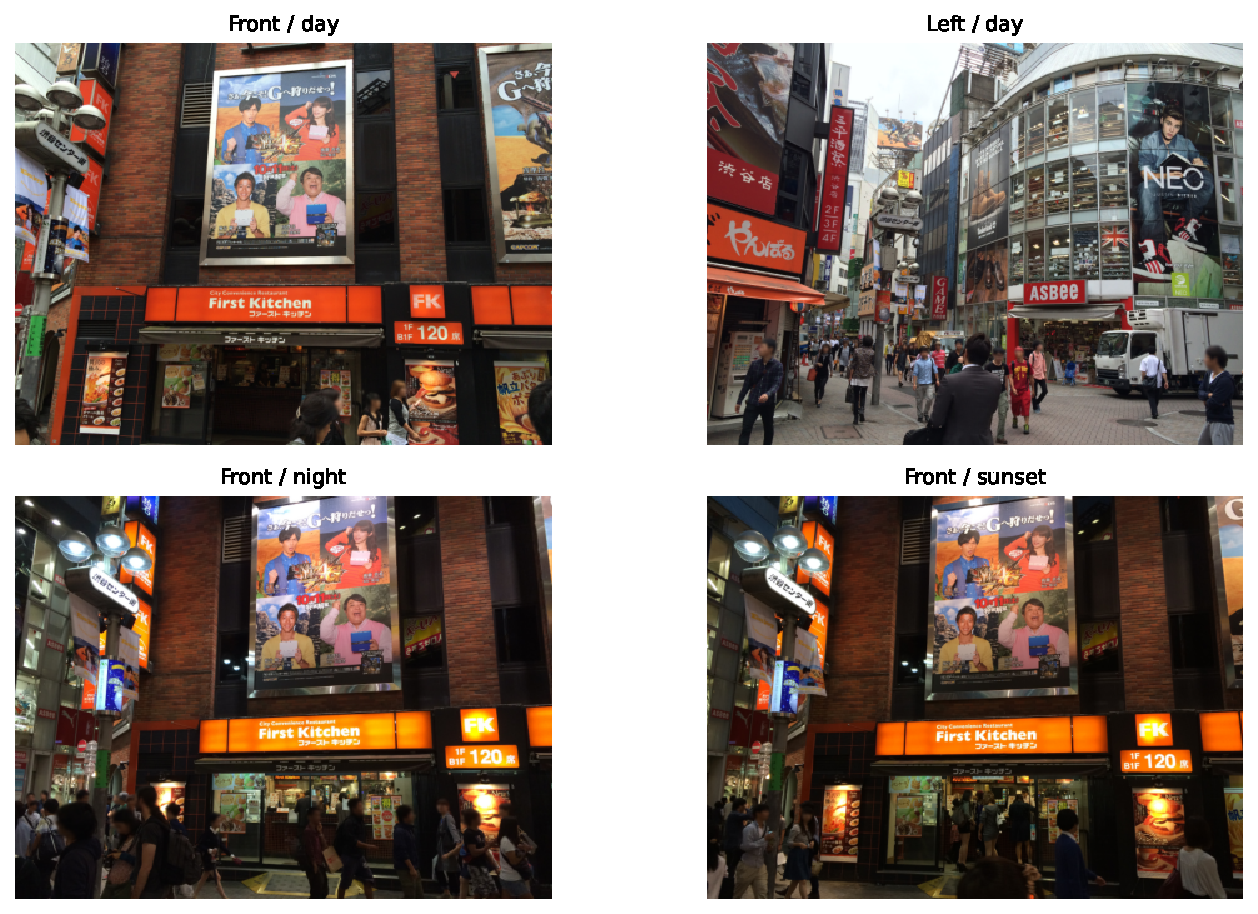
\includegraphics[width=.92\textwidth]{evidence/tokyo_21.pdf}
\caption{All retained photographs for tokyo\_021.}\label{fig:tokyo-scene-21}\end{figure}

\begin{table}[H]\centering\small
\caption{All main-method decisions for tokyo\_021.}\label{tab:tokyo-site-21}
\begin{tabular}{llrlr}\toprule
Protocol & Method & R & Decision & Selected inliers \\
\midrule
D--D & SIFT & 23 & rejected & 0 \\
D--D & SP+LG & 5 & wrong & 14 \\
D--D & Global & 5 & ranking only & -- \\
D--D & Full & 5 & wrong & 14 \\
D--N & SIFT & 1 & correct & 62 \\
D--N & SP+LG & 1 & correct & 201 \\
D--N & Global & 1 & ranking only & -- \\
D--N & Full & 1 & correct & 201 \\
N--D & SIFT & 1 & correct & 60 \\
N--D & SP+LG & 1 & correct & 200 \\
N--D & Global & 1 & ranking only & -- \\
N--D & Full & 1 & correct & 200 \\
D--S & SIFT & 1 & correct & 103 \\
D--S & SP+LG & 1 & correct & 251 \\
D--S & Global & 1 & ranking only & -- \\
D--S & Full & 1 & correct & 251 \\
\bottomrule\end{tabular}\end{table}


Across these four protocols, SIFT correctly verifies 3, exhaustive SP+LG 3, and the full hierarchy 3 of the four queries. The full hierarchy makes 1 wrong-place acceptance and 0 rejections. These counts separate a missing anchor from an incorrectly accepted identity; the latter is the more direct location-association failure.

For this site, the full-pipeline changed-direction daytime query is accepted at the wrong place, while its front-facing day-to-night query is correctly verified. This paired observation should be read with the photographs and the rank column. It does not identify the causal effect of illumination alone, because overlap and view direction also change between the protocols. No corner-error or metric-pose value is inferred from a correct place label.

\section{Site tokyo\_022}

This site contributes four real photographs and four labelled retrieval queries. Each protocol uses one of the photographs as its query and the condition-specific 24-site gallery defined in the frozen benchmark. Reusing a site across protocols produces paired condition observations, not four new geographic locations.

\begin{figure}[H]\centering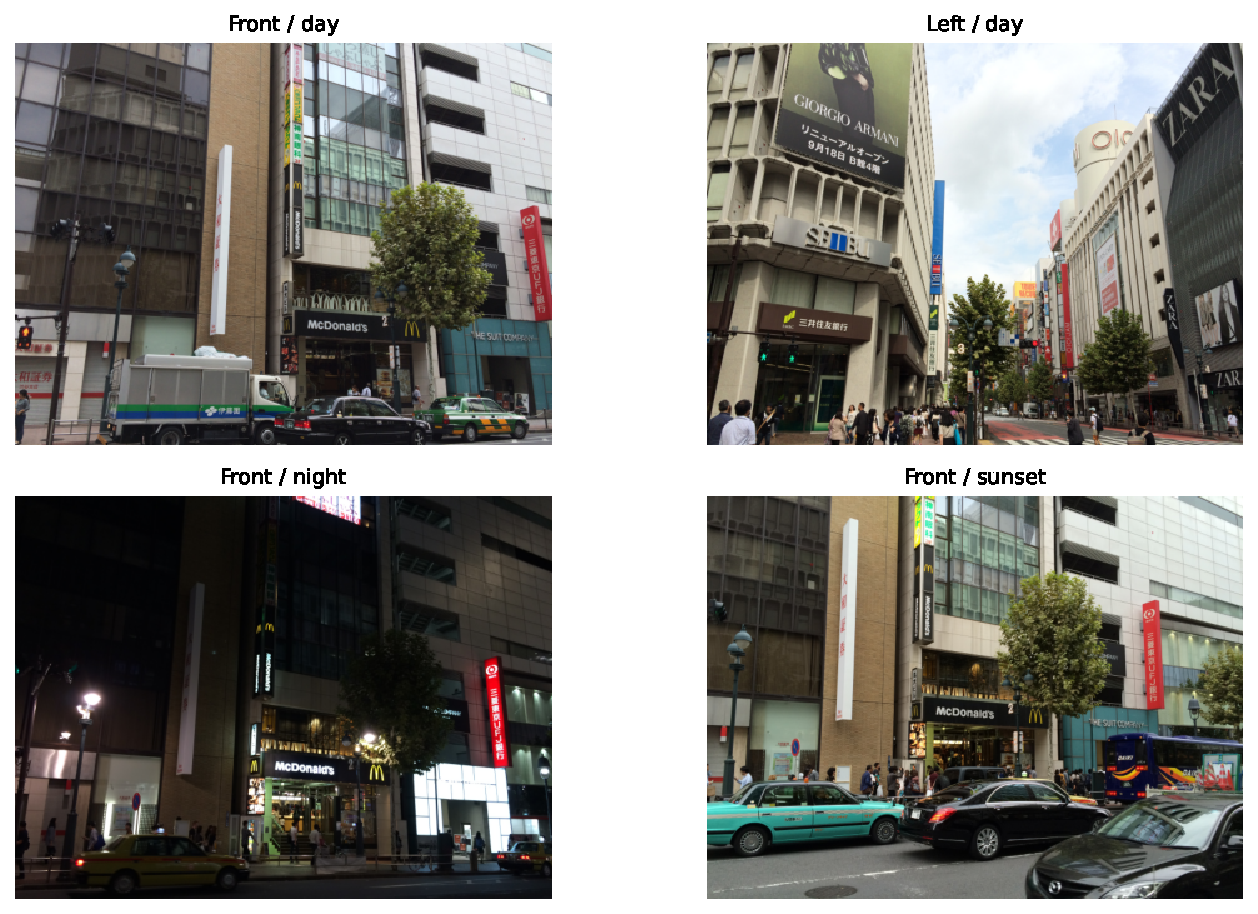
\includegraphics[width=.92\textwidth]{evidence/tokyo_22.pdf}
\caption{All retained photographs for tokyo\_022.}\label{fig:tokyo-scene-22}\end{figure}

\begin{table}[H]\centering\small
\caption{All main-method decisions for tokyo\_022.}\label{tab:tokyo-site-22}
\begin{tabular}{llrlr}\toprule
Protocol & Method & R & Decision & Selected inliers \\
\midrule
D--D & SIFT & 2 & rejected & 0 \\
D--D & SP+LG & 5 & wrong & 13 \\
D--D & Global & 21 & ranking only & -- \\
D--D & Full & 21 & rejected & 0 \\
D--N & SIFT & 1 & rejected & 0 \\
D--N & SP+LG & 1 & correct & 162 \\
D--N & Global & 1 & ranking only & -- \\
D--N & Full & 1 & correct & 162 \\
N--D & SIFT & 9 & rejected & 0 \\
N--D & SP+LG & 1 & correct & 171 \\
N--D & Global & 1 & ranking only & -- \\
N--D & Full & 1 & correct & 171 \\
D--S & SIFT & 1 & correct & 78 \\
D--S & SP+LG & 1 & correct & 198 \\
D--S & Global & 1 & ranking only & -- \\
D--S & Full & 1 & correct & 198 \\
\bottomrule\end{tabular}\end{table}


Across these four protocols, SIFT correctly verifies 1, exhaustive SP+LG 3, and the full hierarchy 3 of the four queries. The full hierarchy makes 0 wrong-place acceptances and 1 rejection. These counts separate a missing anchor from an incorrectly accepted identity; the latter is the more direct location-association failure.

For this site, the full-pipeline changed-direction daytime query is rejected, while its front-facing day-to-night query is correctly verified. This paired observation should be read with the photographs and the rank column. It does not identify the causal effect of illumination alone, because overlap and view direction also change between the protocols. No corner-error or metric-pose value is inferred from a correct place label.

\section{Site tokyo\_023}

This site contributes four real photographs and four labelled retrieval queries. Each protocol uses one of the photographs as its query and the condition-specific 24-site gallery defined in the frozen benchmark. Reusing a site across protocols produces paired condition observations, not four new geographic locations.

\begin{figure}[H]\centering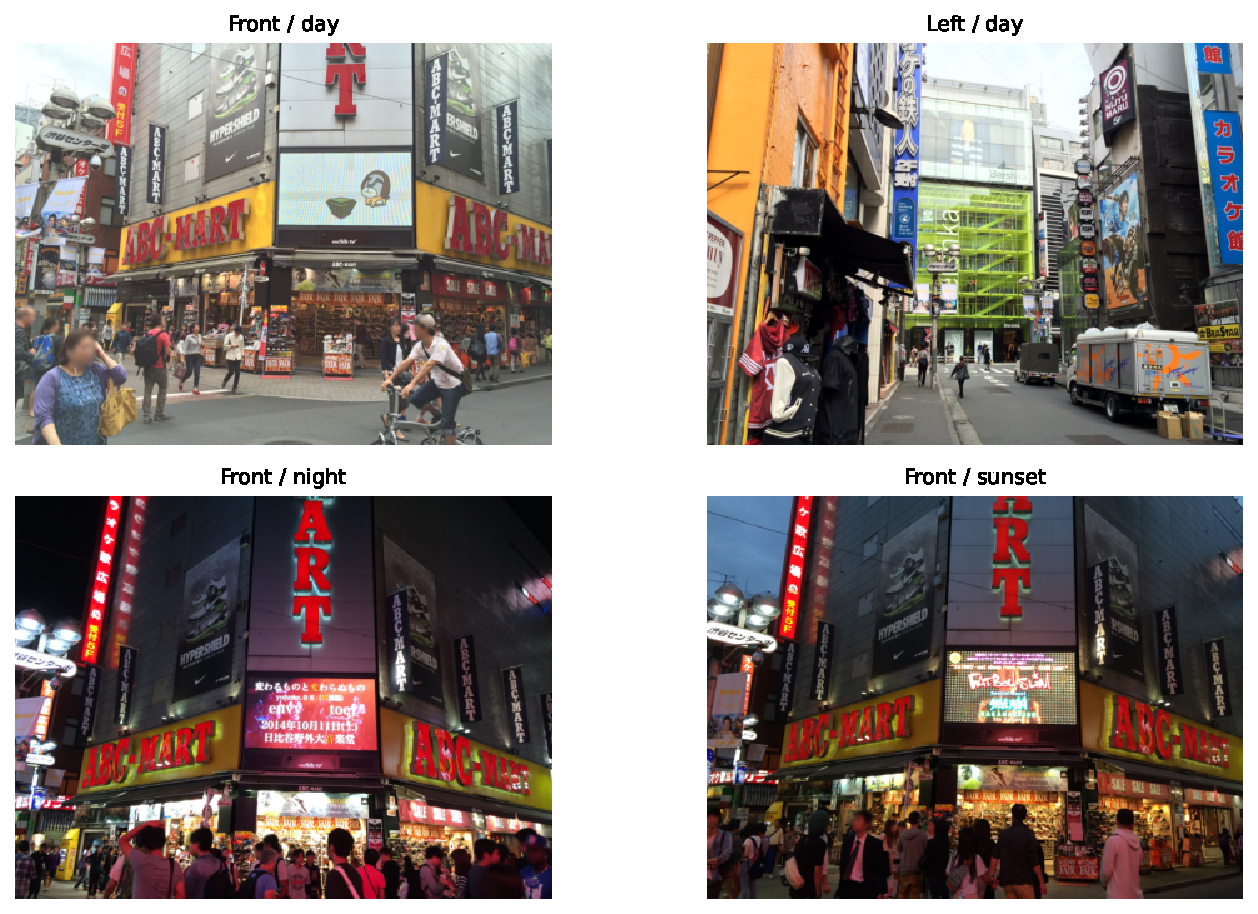
\includegraphics[width=.92\textwidth]{evidence/tokyo_23.pdf}
\caption{All retained photographs for tokyo\_023.}\label{fig:tokyo-scene-23}\end{figure}

\begin{table}[H]\centering\small
\caption{All main-method decisions for tokyo\_023.}\label{tab:tokyo-site-23}
\begin{tabular}{llrlr}\toprule
Protocol & Method & R & Decision & Selected inliers \\
\midrule
D--D & SIFT & 24 & rejected & 0 \\
D--D & SP+LG & 13 & rejected & 0 \\
D--D & Global & 1 & ranking only & -- \\
D--D & Full & 3 & rejected & 0 \\
D--N & SIFT & 2 & rejected & 0 \\
D--N & SP+LG & 1 & correct & 135 \\
D--N & Global & 1 & ranking only & -- \\
D--N & Full & 1 & correct & 135 \\
N--D & SIFT & 3 & rejected & 0 \\
N--D & SP+LG & 1 & correct & 137 \\
N--D & Global & 1 & ranking only & -- \\
N--D & Full & 1 & correct & 137 \\
D--S & SIFT & 1 & rejected & 0 \\
D--S & SP+LG & 1 & correct & 149 \\
D--S & Global & 1 & ranking only & -- \\
D--S & Full & 1 & correct & 149 \\
\bottomrule\end{tabular}\end{table}


Across these four protocols, SIFT correctly verifies 0, exhaustive SP+LG 3, and the full hierarchy 3 of the four queries. The full hierarchy makes 0 wrong-place acceptances and 1 rejection. These counts separate a missing anchor from an incorrectly accepted identity; the latter is the more direct location-association failure.

For this site, the full-pipeline changed-direction daytime query is rejected, while its front-facing day-to-night query is correctly verified. This paired observation should be read with the photographs and the rank column. It does not identify the causal effect of illumination alone, because overlap and view direction also change between the protocols. No corner-error or metric-pose value is inferred from a correct place label.
